% ============================================================
%  MSc Dissertation — Full Document (Expanded)
%  Encoder-Based Policy Guardrails for Autonomous Web Agents
%  Abdulhakim Bashir | MSc Artificial Intelligence
%  University of Essex Online | Supervisor: Dr Diego Navarra
% ============================================================
\documentclass[12pt,a4paper]{article}
\usepackage[utf8]{inputenc}
\usepackage[T1]{fontenc}
\usepackage{times}
\usepackage[margin=2.5cm]{geometry}
\usepackage{setspace}
\usepackage{amsmath,amssymb}
\usepackage{booktabs,array,longtable}
\usepackage{enumitem}
\usepackage{needspace}
\usepackage{listings}
\usepackage{tikz}
\usetikzlibrary{shapes.geometric,arrows.meta,positioning,fit,backgrounds}
\usepackage{pgfplots}
\usepgfplotslibrary{groupplots}
\pgfplotsset{compat=1.18}
\lstset{basicstyle=\small\ttfamily,breaklines=true,frame=single,
        backgroundcolor=\color{gray!8}}
\usepackage[authoryear,round]{natbib}
\usepackage[colorlinks=true,citecolor=blue,urlcolor=blue,
            linkcolor=blue,pdfborder={0 0 0},
            plainpages=false,pdfpagelabels=true]{hyperref}
\usepackage{xcolor}
\usepackage{titlesec}
\titleformat{\section}[block]{\Large\bfseries}{\thesection}{1em}{}
\titleformat{\subsection}[block]{\large\bfseries}{\thesubsection}{1em}{}
\onehalfspacing
\setlength{\parindent}{0pt}
\setlength{\parskip}{7pt}

\begin{document}
\hypersetup{pageanchor=false}

% ── TITLE PAGE ──────────────────────────────────────────────
\begin{titlepage}
\centering\vspace*{3cm}
{\LARGE\bfseries Encoder-Based Policy Guardrails\\[8pt]
for Autonomous Web Agents}\\[2cm]
{\large Abdulhakim Bashir}\\[0.5cm]
{\normalsize MSc Artificial Intelligence}\\[0.3cm]
{\normalsize University of Essex Online}\\[0.3cm]
{\normalsize Supervisor: Dr Diego Navarra}\\[3cm]
{\normalsize \today}\\[2cm]
{\normalsize Submitted in partial fulfilment of the requirements\\
for the degree of Master of Science in Artificial Intelligence}
\end{titlepage}

% ── TABLE OF CONTENTS ───────────────────────────────────────
\pagenumbering{roman}
\setcounter{page}{1}
\tableofcontents
\clearpage

\section*{Abstract}
\addcontentsline{toc}{section}{Abstract}
This dissertation investigates whether a lightweight encoder-based policy
guardrail can improve the safety of autonomous web agents without requiring a
second large language model, full policy recompilation, or modification of the
underlying agent. The research addresses a documented compliance gap in web
agents, where nominal task completion can remain high while policy-compliant
completion collapses under realistic organisational constraints. The study
adopts a mono-method quantitative design. A Policy Compliance Module (PCM)
based on DeBERTa-v3-base is trained on a benchmark-grounded corpus generated
from 375 ST-WebAgentBench tasks across GitLab, SuiteCRM, and ShoppingAdmin.
Each training instance encodes a structured
\texttt{[POLICY]+[CONTEXT]+[ACTION]} triple, with family-level leakage control,
a held-out standard test split, and a harder challenge split used as the main
robustness check. The trained checkpoint is then integrated into a
BrowserGym-compatible wrapper and exercised in a focused live SuiteCRM pilot.
The final PCM achieves near-ceiling standard-test performance
(precision 0.9972, recall 1.0000, F1 0.9986), but the more credible challenge
split is the key result, with precision 1.0000, recall 0.8424, F1 0.9145,
FPR 0.0000, and ROC-AUC 0.9792. A rule-based baseline reaches only 0.3828 F1
on the standard test. The live pilot confirms that the wrapper operates
end-to-end and reduces observed policy violations, but also reveals a
deployment-relevant false positive on \texttt{click Create Account (link)},
leaving the system-level hypothesis inconclusive. The dissertation concludes
that encoder-scale policy guardrails are viable and auditable for enterprise web
agents when training data are benchmark-grounded and evaluation extends beyond
easy held-out splits, but that live calibration and broader multi-task
evaluation remain necessary before stronger deployment claims can be made.
\clearpage

\hypersetup{pageanchor=true}
\pagenumbering{arabic}
\setcounter{page}{1}

% ============================================================
%  CHAPTER 1: INTRODUCTION
% ============================================================
\setcounter{section}{0}
\section{Introduction}
\label{ch:intro}

\subsection{The Problem}

Large language model (LLM) powered autonomous web agents can now navigate browsers, fill forms, execute multi-step workflows, and modify enterprise databases in response to natural-language instructions, without human intervention at each step
\citep{deng2023mind2web,zhou2024webarena,drouin2024workarena}. Where a language model previously produced a recommendation, an agent now executes it.

Adoption is accelerating. McKinsey's 2025 global survey found that 88\% of organisations are regularly using AI in at least one function, and 62\% are at least experimenting with autonomous agents, though only 23\% are actively scaling them \citep{mckinsey2025}. Despite this momentum, Gartner predicts over 40\% of agentic AI projects will be canceled by end of 2027, with governance and compliance cited as the leading barriers \citep{gartner2025}. Capability has advanced rapidly: GPT-4 achieved 14.41\% on WebArena at launch \citep{zhou2024webarena} and subsequent systems have improved substantially \citep{yang2025agentoccam}, yet \citet{xue2025illusion} show that live-website performance remains up to 59\% lower than closed-benchmark scores.

Task completion capability and policy compliance do not improve together. An agent that completes a workflow while exposing a credential, deleting a record without confirmation, or acting on fabricated data has created legal liability and regulatory exposure, regardless of whether the task goal was nominally achieved. \citet{levy2026stwebagentbench} quantify this on ST-WebAgentBench: across three state-of-the-art agents, the average Completion under Policy (CuP) score falls approximately 38\% below the nominal completion rate, and under five or more concurrent policies CuP collapses to 7.1\%. Across sixteen agents on Agent-SafetyBench, the mean safety score is 38.5\% with no agent above 60\% \citep{zhang2024agentsafety}. The compliance deficit is structural.

Three existing remedy categories each fall short. Training-time alignment methods such as RLHF \citep{ouyang2022training} and Constitutional AI \citep{bai2022constitutional} embed constraints in model weights, cannot adapt to policy changes without retraining, and produce no per-action audit trail. LLM-based runtime guardrails including GuardAgent \citep{xiang2024guardagent}, AGrail \citep{luo2025agrail}, and ShieldAgent \citep{chen2025shieldagent} offer strong accuracy but require 7 to 70 billion-parameter inference engines that introduce 300 to 500\,ms latency per action, incompatible with synchronous pre-execution gating. Deterministic compilation approaches such as ToolGuard \citep{zwerdling2025toolguard} provide sub-millisecond execution and strong auditability, but require complete offline recompilation and expert code review for every policy change and have been evaluated on a single domain with 14 tools only. No existing system simultaneously achieves modularity, encoder-scale inference latency, policy generalisability without recompilation, and per-action auditability across multiple enterprise domains.

\subsection{Research Questions}
\label{sec:rq}

This dissertation is structured around three research questions that collectively
address the design, intrinsic performance, and system-level impact of the
proposed Policy Compliance Module:

\begin{description}[leftmargin=2em,labelindent=0.5em]
  \item[RQ1 (Design):] How can a learned policy compliance module be designed and integrated into a BrowserGym-compatible web agent loop to enforce operational constraints without requiring modification to the underlying agent?
  \item[RQ2 (Classifier Performance):] How accurately can a fine-tuned DeBERTa-v3-base encoder detect policy violations from agent action-context pairs across the six ST-WebAgentBench safety dimensions, and what precision-recall trade-offs arise at different violation thresholds?
  \item[RQ3 (System Evaluation):] Does integrating the PCM produce a statistically significant improvement in Completion under Policy scores on ST-WebAgentBench, at what cost to task completion rate, and does compliance training on synthetic data generalise to real benchmark scenarios?
\end{description}
RQ1 is the primary engineering design question. RQ2 operationalises 
the classifier's intrinsic performance. RQ3 provides the end-to-end 
system-level evidence and validates the data strategy, directly 
addressing the compliance deficit identified by 
\citet{levy2026stwebagentbench}.

\subsection{Aim and Objectives}
\label{sec:aims}

\textbf{Aim:} To develop and evaluate a learned Policy Compliance Module (PCM)
that intercepts autonomous agent actions, assesses them against enterprise
policies, and blocks violations before execution, as measured by Completion under
Policy scores on ST-WebAgentBench \citep{levy2026stwebagentbench} relative to an
unguarded baseline, while maintaining a task completion rate penalty of at most
5\% absolute.

\begin{longtable}[l]{@{} c l p{8.5cm} @{}}
\caption{Project objectives and deliverables}\label{tab:obj}\\
\toprule \textbf{O} & \textbf{Label} & \textbf{Deliverable} \\ \midrule
\endfirsthead
\toprule \textbf{O} & \textbf{Label} & \textbf{Deliverable} \\ \midrule
\endhead \bottomrule \endfoot
O1 & Policy Taxonomy & Documented mapping of ST-WebAgentBench's six safety
  dimensions to parameterised YAML policy templates, defining allowed and
  disallowed action types and context conditions for synthetic data generation
  \citep{levy2026stwebagentbench}. \\[3pt]
O2 & Benchmark-Grounded Corpus & Python codebase producing a benchmark-grounded
  corpus of labelled \texttt{[POLICY]+[CONTEXT]+[ACTION]} triples from
  ST-WebAgentBench task and policy metadata, with family-level split control,
  challenge-set construction, and class balance monitoring
  \citep{li2023synthetic,nadas2025synthetic}. \\[3pt]
O3 & Trained PCM & Fine-tuned DeBERTa-v3-base classifier achieving precision
  $\geq 0.85$, recall $\geq 0.80$, macro-F1 $\geq 0.82$, with model weights
  and training configuration retained for reproducibility
  \citep{he2023debertav3}. \\[3pt]
O4 & System Integration & \texttt{PolicyCompliantAgent} BrowserGym-compatible
  wrapper with configurable threshold $\theta$, multi-policy OR-logic,
  per-action decision logging satisfying EU AI Act Article~12, and optional
  re-planning on blocked actions \citep{chezelles2025browsergym}. \\[3pt]
O5 & Empirical Evaluation & Quantitative analysis combining offline
  benchmark-grounded classifier evaluation, rule-based baseline comparison,
  threshold analysis, and a focused live SuiteCRM pilot using the BrowserGym
  integration harness \citep{mcnemar1947note}. \\[3pt]
O6 & Threshold Analysis & Full precision-recall curves and compliance-utility
  trade-off plots across $\theta \in \{0.10, 0.20, \ldots, 0.99\}$. \\[3pt]
O7 & Robustness Assessment & Held-out challenge-set evaluation and qualitative
  live pilot analysis quantifying the gap between in-distribution offline
  performance and behaviour in a live SuiteCRM agent loop. \\
\end{longtable}

Objectives O1--O5 are essential and correspond directly to the primary hypotheses.
O6 and O7 are secondary objectives that may be partially addressed subject to
time constraints, consistent with the approved research proposal.

\subsection{Working Hypotheses}
\label{sec:hyp}

Following the deductive approach, the following hypotheses operationalise the
research questions for empirical testing \citep{saunders2019research}:

\begin{longtable}[l]{@{} c c p{9cm} @{}}
\caption{Working hypotheses aligned to research questions}\label{tab:hyp}\\
\toprule \textbf{H} & \textbf{RQ} & \textbf{Hypothesis} \\ \midrule
\endfirsthead
\toprule \textbf{H} & \textbf{RQ} & \textbf{Hypothesis} \\ \midrule
\endhead \bottomrule \endfoot
H1 & 2 & A fine-tuned DeBERTa-v3-base classifier can detect policy violations
  from action-context pairs with precision $\geq 0.85$ and recall $\geq 0.80$,
  consistent with the encoder advantage over zero-shot LLMs documented by
  \citet{bucher2024finetuned} and the safety classification efficiency
  demonstrated by \citet{zheng2025lightweight}. \\[4pt]
H2 & 3 & Integrating the PCM with baseline agents will improve CuP scores by
  $\geq 10\%$ relative to unguarded baseline agents on ST-WebAgentBench,
  addressable within the $\approx 38\%$ compliance gap identified by
  \citet{levy2026stwebagentbench}, with task completion rate declining by
  $\leq 5\%$ absolute. \\[4pt]
H3 & 2 & Increasing the violation threshold $\theta$ will increase task
  completion rates while decreasing policy compliance rates, exhibiting a
  monotonic and measurable trade-off demonstrable through precision-recall curves;
  and a classifier trained on benchmark-grounded policy-violation data will
  retain at least 70\% of its held-out test performance on a harder challenge
  split and limited live benchmark scenarios, consistent with generalisation evidence for
  LLM-generated structured data reported by \citet{li2023synthetic}. \\
\end{longtable}

H1 and H2 are primary success criteria whose joint satisfaction constitutes
validation of the PCM's core claims. H3 provides secondary insights into
threshold behaviour and data strategy validity.

\subsection{Background}
\label{sec:background}

\subsubsection{From Scripted Automation to Language-Driven Agents} RPA tools achieve reliable performance on stable workflows but cannot interpret natural-language instructions or generalise beyond scripted coverage. LLM-based agents overcome this through generalisation, enabling action selection across novel environments without task-specific programming \citep{deng2023mind2web,zhou2024webarena,drouin2024workarena}. This same capability creates governance risk: an LLM agent can take actions that are contextually plausible but operationally impermissible. 

\subsubsection{The Enterprise Compliance Environment}

Enterprise agents operate within multi-dimensional, policy-governed contexts
across the three platforms evaluated in ST-WebAgentBench
\citep{levy2026stwebagentbench}. These constraints are formalised through
six orthogonal safety dimensions: User Consent, Boundary and Scope, Strict
Execution, Hierarchy Adherence, Robustness and Security, and Error Handling.
Each dimension can be violated independently and contributes to the CuP
penalty. Chapter~2 examines each dimension in detail.

\subsubsection{Why Compliance Cannot Be Delegated to the Base Agent}

Four structural reasons explain why compliance cannot be embedded in the base agent. First, the compliance gap persists across frontier alignment-trained models \citep{levy2026stwebagentbench}, confirming that general alignment does not produce enterprise-grade policy compliance. Second, enterprise policies are dynamic and change continuously; weight-embedded compliance requires full retraining to adapt. Third, EU AI Act Article~12 \citep{euaiact2024} mandates per-action audit records that no training-time method produces. Fourth, the agent and compliance function serve different organisational principals with different update cycles, making a modular separation architecturally essential.

\subsubsection{The Proposed Approach} The PCM operates between planning and execution. When the base agent proposes an action, the PCM intercepts it, forms a structured \texttt{[POLICY]+[CONTEXT]+[ACTION]} triple, and runs a forward pass through fine-tuned DeBERTa-v3-base \citep{he2023debertav3} to produce $P(\text{violation})$. Actions exceeding threshold $\theta$ are blocked before reaching the browser. The architecture requires no modification to the base agent and integrates as a modular wrapper into any BrowserGym-compatible loop \citep{chezelles2025browsergym}. 

\subsection{Regulatory Context}
\label{sec:regulatory}

The PCM's architecture is directly aligned with binding governance requirements
that apply from August 2026 to high-risk AI system deployers. The EU AI Act
\citep{euaiact2024} mandates automatic logging of all events during high-risk AI
system operation (Article~12), transparency documentation enabling deployers to
interpret AI outputs (Article~13), human oversight measures with operator override
capability (Article~14), and lifecycle risk management systems (Article~9). The
PCM's per-action audit log, continuous probability score, configurable blocking
threshold, and modular architecture directly operationalise each of these
obligations. The NIST AI Risk Management Framework \citep{nist2023rmf} and
ISO/IEC~42001:2023 \citep{iso2023} provide complementary governance requirements
that the PCM satisfies through its measurable performance metrics and event
logging infrastructure.

\subsection{Contributions} This dissertation makes three contributions. First, it designs and implements the PCM, an encoder-based pre-execution compliance classifier integrated into a BrowserGym-compatible agent loop. Second, it provides empirical evidence that an encoder-scale classifier at approximately 86M parameters can achieve strong benchmark-grounded offline policy-violation detection, including a harder held-out challenge split that is materially more credible than a near-ceiling standard test set. Third, it contributes a reproducible benchmark-grounded data construction and evaluation pipeline that converts ST-WebAgentBench policy and task metadata into runtime-shaped training examples without requiring proprietary enterprise logs.

The remainder of the dissertation is structured as follows. Chapter~2 reviews
the literature on web-agent benchmarks, policy-compliance failures, and the
trade-offs between training-time, rule-based, and runtime guardrail approaches.
Chapter~3 explains the research design, benchmark-grounded data strategy, and
evaluation protocol. Chapter~4 presents the PCM architecture, model-training
configuration, and BrowserGym integration. Chapter~5 reports and interprets the
offline and live evaluation results. Chapter~6 discusses the implications,
limitations, generalisability, and future directions of the study.
% ============================================================
%  CHAPTER 2: LITERATURE REVIEW
% ============================================================
\newpage
\setcounter{section}{1}
\section{Literature Review}
\label{ch:litreview}

The PCM sits at the intersection of five literatures: web-agent capability,
agent safety, AI governance, transformer-based classification, and the false
positive problem in automated compliance systems. This chapter reviews each area
selectively rather than exhaustively, focusing on what is needed to justify the
artefact design and the evaluation strategy.

The review draws primarily on peer-reviewed work from ICLR, ICML, NeurIPS, ACL,
EMNLP, NAACL, COLING, USENIX Security, and TMLR. Pre-prints are used only where
they represent the most current and field-shaping evidence on a rapidly moving
topic, especially frontier web agents and runtime guardrails.

%--------------------------------------------------------------
\subsection{Web Agent Architectures and Capabilities}
%--------------------------------------------------------------

General-purpose web agents became practical with benchmarks such as Mind2Web,
WebArena, and VisualWebArena, which together established cross-site
generalisation, long-horizon interaction, and multimodal grounding as the core
capability challenges \citep{deng2023mind2web,zhou2024webarena,koh2024visualwebarena}.
Mind2Web was especially important methodologically because it introduced
cross-split generalisation and the now-standard two-stage pattern in which a
smaller model narrows candidate elements before a larger model selects the
action. WebArena then moved the field toward executable, self-hosted
environments with functional task evaluation, making it possible to measure
full trajectories rather than static next-step prediction.

Consumer-web benchmarks, however, do not fully capture enterprise workflows.
WorkArena translates the web-agent problem into structured ServiceNow tasks,
including multi-step compositional workflows in which one early mistake can
invalidate all later progress \citep{drouin2024workarena}. That failure mode is
important for this dissertation because it mirrors the logic of compliance:
under ST-WebAgentBench, one policy violation can nullify an otherwise successful
trajectory. BrowserGym provides the common interface that makes such comparisons
possible. Its standardised observation and action spaces separate planning from
execution cleanly enough that a compliance mechanism can be inserted between
them without changing the base agent \citep{chezelles2025browsergym}.

This enterprise turn matters conceptually as well as practically. Earlier web
benchmarks showed that long-horizon browser control is difficult; WorkArena and
BrowserGym showed that the same difficulty persists once workflows become
permissioned, stateful, and operationally consequential. The PCM therefore sits
within a broader shift from ``can the agent finish the task?'' to ``can it
finish the task without violating constraints that matter to an organisation?''.

Three further findings matter directly for PCM design. First, grounding remains
a decisive bottleneck. SeeAct shows that performance can jump sharply when
element grounding is made more reliable, implying that action semantics are best
captured after grounding rather than from raw element identifiers alone
\citep{zheng2024seeact}. Second, representation design matters materially.
AgentOccam demonstrates that even without changing the base model, restructuring
the AXTree to better fit pre-training distributions can produce large gains
\citep{yang2025agentoccam}. Third, benchmark scores overstate deployment
readiness. \citet{xue2025illusion} report that performance on live websites can
drop dramatically relative to closed-benchmark scores, which is exactly why a
policy guardrail should be judged on more than an easy in-distribution test.

This literature leaves two gaps. Most mainstream web-agent papers still treat
task completion as the end metric, and none evaluates an encoder-scale
pre-execution guardrail integrated into the live control loop
\citep{zhou2024webarena,drouin2024workarena,chezelles2025browsergym}.

%--------------------------------------------------------------
\subsection{Agent Safety and Policy Compliance}
%--------------------------------------------------------------

Training-time alignment methods such as RLHF and Constitutional AI improve
general harmlessness, but they are poorly suited to enterprise policy
compliance. Their constraints are embedded in model weights, difficult to update
when local policy changes, and they do not natively produce a per-action record
of which policy was checked against which action
\citep{ouyang2022training,bai2022constitutional,euaiact2024}. That is a serious
misfit for enterprise settings in which policies change continuously and audit
trails are a first-class requirement rather than an optional feature.

The strongest direct evidence for the compliance problem comes from
ST-WebAgentBench \citep{levy2026stwebagentbench}. The benchmark covers 375 tasks
and 3,057 policy instances across six dimensions: User Consent, Boundary and
Scope, Strict Execution, Hierarchy Adherence, Robustness and Security, and Error
Handling. Its key metric is Completion under Policy:
\begin{equation}
\text{CuP}_t = C_t \times \mathbf{1}\!\left[\sum_{d} V^t_d = 0\right], \quad
\text{CuP} = \frac{1}{T}\sum_{t=1}^{T}\text{CuP}_t
\label{eq:cup}
\end{equation}
Across the published agents, CuP falls materially below nominal completion, and
under heavier policy load it degrades even further. In other words, task success
and policy compliance do not move together. The benchmark is also useful
analytically because it identifies the dominant failure sources: User Consent
and Strict Execution account for most violations, while the explicit policy
hierarchy formalises the precedence of organisational constraints over user- or
task-level instructions. ST-WebAgentBench is therefore not just a benchmark but
the clearest empirical statement of the operational problem this dissertation
addresses.

The benchmark is also unusually informative about scale and structure. Its task
set spans GitLab, ShoppingAdmin, and SuiteCRM, with the latter further broken
into Easy, Medium, and Hard subsets with increasing policy density
\citep{levy2026stwebagentbench}. The published results show that compliance does
not fail only on rare corner cases. Average completion remains materially above
average CuP, partial completion outstrips fully compliant completion by an even
larger margin, and all-pass@3 scores remain low, revealing substantial
run-to-run brittleness. This matters because it rules out a comforting
interpretation in which violations are merely occasional slips by otherwise
stable agents. Instead, the benchmark suggests a structural mismatch between
what current agents optimise for and what enterprise deployment requires.

Complementary safety work points in the same direction. Agent-SafetyBench shows
that current agents remain far from robust safety performance even beyond web
automation \citep{zhang2024agentsafety}. Runtime guardrail work then clarifies
the design space. GuardAgent and AGrail retain semantic flexibility through
LLM-based checks but pay substantial inference cost
\citep{xiang2024guardagent,luo2025agrail}. ShieldAgent and ToolGuard reduce
runtime overhead through compilation or rule execution, but at the cost of
rebuild overhead, narrower policy adaptability, or limited domain coverage
\citep{chen2025shieldagent,zwerdling2025toolguard}. This is the architectural
opening for the PCM --- a smaller learned classifier that stays semantic,
modular, and cheap enough for synchronous gating.

The details of these systems strengthen that conclusion. GuardAgent uses a
knowledge-enabled LLM guard that can interpret natural-language constraints but
still incurs a full generative pass for each decision \citep{xiang2024guardagent}.
AGrail improves robustness, including against environmental prompt injection,
but does so through a cooperative multi-LLM architecture whose runtime cost is
still far above that of an encoder classifier \citep{luo2025agrail}. By
contrast, ShieldAgent and ToolGuard move toward deterministic execution through
compiled policy logic and tool guards \citep{chen2025shieldagent,zwerdling2025toolguard}.
That improves auditability and latency, but it also makes policy evolution more
expensive because policy change implies rebuild or recompilation. The PCM is
therefore best understood as occupying the middle ground between flexible but
slow LLM guards and fast but rigid compiled guards.

\begin{table}[htbp]
\centering\small
\caption{Comparison of runtime guardrail approaches against PCM requirements}
\label{tab:guardrail_comparison}
\begin{tabular}{@{} l c c c c c @{}}
\toprule
\textbf{System} & \textbf{Modular} & \textbf{Low latency} & \textbf{No rebuild} & \textbf{Auditability} & \textbf{Multi-domain} \\
\midrule
GuardAgent \citep{xiang2024guardagent}   & Yes & No  & Yes & Limited & Limited \\
AGrail \citep{luo2025agrail}             & Yes & No  & Yes & Limited & Yes \\
ShieldAgent \citep{chen2025shieldagent}  & Yes & Yes & No  & Yes     & Limited \\
ToolGuard \citep{zwerdling2025toolguard} & Yes & Yes & No  & Yes     & No \\
\midrule
\textbf{PCM (proposed)} & Yes & Yes & Yes & Yes & Yes \\
\bottomrule
\end{tabular}
\end{table}

The comparison in Table~\ref{tab:guardrail_comparison} motivates the chosen
positioning. The PCM is not intended to outperform every alternative on every
dimension. Rather, it targets the specific intersection that the current
literature leaves underserved: semantic policy interpretation at encoder-scale
latency with per-action logging and no offline recompilation.

%--------------------------------------------------------------
\subsection{Enterprise AI Governance and Regulatory Frameworks}
%--------------------------------------------------------------

The governance literature reinforces the technical case for a modular guardrail.
The EU AI Act requires risk management, logging, transparency, and human
oversight for high-risk AI systems \citep{euaiact2024}. The NIST AI RMF and its
Generative AI Profile emphasise measurable evaluation, semantic filtering, and
traceable risk controls \citep{nist2023rmf,autio2024nist}. ISO/IEC~42001
similarly treats monitored performance and event logging as management-system
requirements rather than optional best practice \citep{iso2023}. OWASP's 2025
Top~10 for LLM applications adds an attack-oriented perspective, especially
prompt injection and excessive agency \citep{owasp2025llm}.

These frameworks do not prescribe an encoder-based solution, but they do imply
four concrete design requirements: intervention before execution, operator
visibility into the decision, reconfigurability without full model retraining,
and durable event logging. This alignment matters because it shows the PCM is
not just technically convenient; it is a direct response to external governance
expectations now shaping enterprise AI deployment.

The governance perspective also sharpens the distinction between compliance and
general alignment. General alignment asks whether a model tends to behave
helpfully or harmlessly across broad situations. Governance frameworks ask
whether a deployer can document, inspect, justify, and override system behaviour
under specific operational controls. That distinction is one reason the PCM is
architected as a separate module instead of an assumption about the base agent's
intrinsic trustworthiness.

%--------------------------------------------------------------
\subsection{Transformer-Based Text Classification for Policy Detection}
%--------------------------------------------------------------

The PCM draws on the standard pre-train/fine-tune paradigm established by BERT
and refined by RoBERTa and DeBERTa \citep{devlin2019bert,liu2019roberta,he2021deberta}.
DeBERTa-v3 is especially relevant because its disentangled attention suits
structured segment inputs, while its replaced-token-detection objective inherits
the efficiency advantages of ELECTRA-style pre-training
\citep{he2023debertav3,clark2020electra}. That combination is a good fit for a
classifier that must reason over explicitly delimited policy, context, and
action segments rather than over free-form prose alone.

The broader classification literature supports the model choice directly.
Fine-tuned encoders consistently outperform zero-shot generative LLMs on
specialised classification tasks, especially when the label space is narrow but
the decision boundary is domain-specific
\citep{bucher2024finetuned,galke2025texclassification}. This matters because
policy compliance is exactly such a task: binary in output, but highly specific
in how the positive class is defined. Recent safety work also shows that
lightweight encoders can approach much larger guardrail systems at far lower
runtime cost \citep{zheng2025lightweight}. That is the deployment niche the PCM
targets.

DeBERTa-v3 is also attractive for a more specific reason: its gains are
especially notable in low-resource classification settings
\citep{he2023debertav3}. That matters here because policy-violation data are not
available at internet scale; even a benchmark-grounded corpus remains small by
modern pre-training standards. The objective is not to discover a general web
agent from scratch, but to specialise a mature encoder to a narrow and
operationally meaningful distinction. In that regime, the literature strongly
favours supervised fine-tuning of compact encoders over prompting much larger
generative models.

There is nevertheless an architectural trade-off. Newer encoders such as
ModernBERT promise longer context windows and more modern attention machinery
\citep{warner2024modernbert}. For this dissertation, however, the main
bottleneck is not thousand-token document understanding; it is reliable
classification of short structured triples under moderate data and latency
constraints. The final design therefore prioritises DeBERTa-v3's empirical
strength in supervised classification over newer but less validated choices for
this exact use case.

Because real policy-violation corpora are scarce, synthetic or benchmark-derived
augmentation is unavoidable. Prior work shows that synthetic data can support
objective classification tasks when labels are logically determined and quality
controls are explicit \citep{anabytavor2020data,li2023synthetic,nadas2025synthetic}.
The key methodological lesson is not that any synthetic data will do, but that
generation quality and split design are decisive. This is why the final corpus
in this dissertation is benchmark-grounded and family-split rather than a small
templated sentence set.

This point is especially important because synthetic-data results are easy to
overclaim. The literature is clear that synthetic augmentation is strongest when
the target predicate is explicit and verifiable, not when labels depend on vague
human preference \citep{li2023synthetic,nadas2025synthetic}. Policy compliance
fits that better than many other safety tasks because the central question is
whether an action violates a stated policy. Even so, generation shortcuts can
still create unrealistically separable splits. That observation directly
motivates the challenge set and the insistence in Chapter~5 on treating the
harder split, not the near-ceiling standard split, as the more credible
indicator of generalisation.

%--------------------------------------------------------------
\subsection{The False Positive Problem in Compliance Systems}
%--------------------------------------------------------------

False positives are not a minor operational inconvenience. In security
operations, high false-positive rates create alert fatigue, reduced trust, and
eventual abandonment of the monitoring system \citep{alahmadi2022fps}. In AML,
rule-based monitoring likewise produces large volumes of benign alerts, which is
why learned screening approaches are increasingly preferred
\citep{ghimire2025aml}. For an autonomous-agent guardrail, the consequence is
sharper still --- a false positive can directly fail or delay the task. That is
why precision and FPR are treated in this dissertation as co-equal with recall,
not secondary reporting metrics.

There is also an evaluation lesson. \citet{movva2024annotation} show that safety
labelling can be genuinely ambiguous when it depends on human normative
judgement. Policy-compliance classification is more objective than
conversational safety annotation because the predicate is tied to an explicit
policy statement, but the general lesson still holds: ambiguous or transitional
cases should be inspected qualitatively, not hidden beneath headline averages.

That insight becomes concrete in the live SuiteCRM pilot reported later. The
offline classifier performs strongly, but a transitional action such as
\texttt{click Create Account (link)} can still be misread when the active policy
is framed around eventual save behaviour. This is not a reason to abandon the
approach; it is evidence that live false positives should feed back into corpus
design and calibration rather than being dismissed as anecdotal noise.

%--------------------------------------------------------------
\subsection{Synthesis and Research Gap}
\label{sec:synthesis}
%--------------------------------------------------------------

Taken together, the literature establishes five points. First, web agents are
becoming more capable, but benchmark success still overstates live reliability
\citep{xue2025illusion}. Second, the compliance gap is structural and is
quantified most clearly by ST-WebAgentBench \citep{levy2026stwebagentbench}.
Third, governance frameworks require logging, transparency, and human oversight
\citep{euaiact2024,nist2023rmf,iso2023}. Fourth, fine-tuned encoders are both
strong and efficient on specialised classification
\citep{bucher2024finetuned,zheng2025lightweight}. Fifth, false positives are
operationally costly enough to be a first-order design constraint
\citep{alahmadi2022fps,ghimire2025aml}. What is still missing is a modular,
benchmark-grounded, encoder-scale pre-execution guardrail evaluated against this
combined set of technical, governance, and operational requirements. That gap
defines the contribution of the PCM.


% ============================================================
%  CHAPTER 3: METHODOLOGY
% ============================================================
\newpage
\setcounter{section}{2}
\section{Methodology}
\label{ch:methodology}

This chapter presents the methodological framework governing the design, data
collection, and evaluation of the PCM. It is organised around three principal
concerns: philosophical and strategic positioning within a formal research
tradition; the two-pronged data collection strategy; and the experimental design,
evaluation metrics, and statistical analysis plan. The chapter concludes with
ethical and professional considerations. Throughout, methodological choices are
explicitly justified with reference to the research questions and prior literature
rather than asserted as convention.

%--------------------------------------------------------------
\subsection{Research Philosophy and Design}
%--------------------------------------------------------------

\subsubsection{Philosophical Position: Positivism}

This research adopts a positivist philosophical position. Positivism holds that
reality is objective and measurable independently of the researcher, and that
knowledge advances through the systematic empirical testing of propositions against
observable data \citep{saunders2019research,bryman2016social}. This position is
appropriate for the present research for three specific reasons. First, all primary
research questions require quantitative measurement: classifier precision, recall,
and F1 score; Completion under Policy scores; per-dimension false positive rates;
and inference latency measurements. These are objective metrics with established
definitions that can be computed consistently regardless of researcher identity.
Second, the experimental environment (ST-WebAgentBench) running on identical
hardware with identical agent configurations is reproducible, and conditions
can be held constant across configurations, enabling the controlled comparisons
that positivism prescribes. Third, the hypotheses are formulated as specific,
falsifiable predictions derived from prior theoretical and empirical work,
consistent with the hypothetico-deductive model characteristic of positivist
inquiry \citep{bryman2016social}.

Interpretivism is unsuitable as the research concerns measurable software performance rather than subjective meaning-making or social phenomena.

\subsubsection{Research Approach: Deductive}

The research follows a deductive approach, deriving testable hypotheses from
established theoretical premises that that fine-tuned encoders outperform LLMs
for specialised classification \citep{bucher2024finetuned}, that the compliance
gap is measurable \citep{levy2026stwebagentbench}, and that synthetic data is
viable for objective classification \citep{li2023synthetic}, and testing them
through controlled benchmark experiments. H1--H3 (Table~\ref{tab:hyp}) specify
the predictions; Chapters~4 and~5 report their empirical evaluation.

\subsubsection{Research Strategy: Design Science Research}

The primary research strategy is Design Science Research (DSR)
\citep{hevner2004design}, which is concerned with the creation and rigorous
evaluation of purposeful IT artefacts to address identified organisational
problems.  DSR is appropriate because the primary contribution is a technical artefact
rather than a theoretical explanation \citep{march1995design}. The research
follows \citet{peffers2007dsrm}'s six-stage DSRM:

\begin{enumerate}[noitemsep,leftmargin=2em]
  \item \textbf{Problem identification:} the $\sim$38\% CuP compliance gap
    \citep{levy2026stwebagentbench}.
  \item \textbf{Objective definition:} H1 and H2 performance thresholds and
    objectives O1--O5 from Table~\ref{tab:obj}.
  \item \textbf{Design and development:} encoder selection, data pipeline,
    and BrowserGym wrapper, detailed in Chapter~4.
  \item \textbf{Demonstration:} integration with ST-WebAgentBench via the
    \texttt{PolicyCompliantAgent} wrapper.
  \item \textbf{Evaluation:} controlled benchmark experiments across four
    configurations, reported in Chapter~5.
  \item \textbf{Communication:} this dissertation and open-source code
    repository released under MIT licence.
\end{enumerate}

Evaluation follows \citet{venable2016feds}'s FEDS framework using ex-post
naturalistic benchmark experimentation.

\subsubsection{Methodological Choice: Mono-Method Quantitative}

The research employs a mono-method quantitative design, collecting exclusively
numerical data through a single evaluation framework \citep{saunders2019research}.
This choice is justified by three considerations. First, the technical nature of
the research questions: RQ1--RQ3 all require measurable system performance metrics
rather than qualitative accounts of user experience or social meaning. Second, the
existence of a standardised evaluation benchmark that eliminates the need for
researcher-designed measurement instruments and enables direct comparison with
published baselines. Third, time constraints and the focused scope of the project:
mixed-methods or multi-method quantitative designs would add considerable data
collection and analysis overhead without materially improving the validity of
answers to the specific research questions posed. Future work incorporating
qualitative validation with enterprise compliance practitioners is identified as a
valuable extension.

%--------------------------------------------------------------
\subsection{Data Collection Strategy}
%--------------------------------------------------------------

Labelled policy-violation data for web agents remains scarce, and no public
dataset provides enough action-policy examples in the exact format required by
the PCM. The final data strategy therefore grounds the training corpus directly
in ST-WebAgentBench task and policy metadata rather than relying on a small
hand-written synthetic set. The key idea is to preserve the benchmark's
taxonomy, applications, and policy semantics while generating actions whose
surface forms resemble the runtime actions the wrapper actually classifies.
This reduces one important source of bias---training on examples that look
nothing like runtime actions---but it does not make the corpus neutral. The
resulting dataset is still a measurement instrument whose definition of
``policy violation'' is inherited from the benchmark itself
\citep{jacobs2021measurement}. It also inherits representation and framing risks
from the benchmark's task mix and policy distribution
\citep{suresh2021harm}. Bias is therefore treated here as a validity issue to
be surfaced and bounded, not as a problem solved by synthetic scale alone.

\subsubsection{Benchmark-Grounded Corpus Construction}

The corpus is generated from the local ST-WebAgentBench task catalogue
(\texttt{test.raw.json}), which contains 375 tasks across SuiteCRM, GitLab, and
ShoppingAdmin \citep{levy2026stwebagentbench}. For each task-policy pair, the
generator derives:

\begin{enumerate}[noitemsep,leftmargin=2em]
  \item a normalised natural-language policy statement;
  \item a structured context string containing site, task ID, module, intent,
    and selected policy metadata; and
  \item matched compliant and violating action strings in BrowserGym-shaped
    natural language.
\end{enumerate}

This produces the same \texttt{[POLICY]+[CONTEXT]+[ACTION]} representation used
by the classifier at training and inference time, while avoiding dependence on
proprietary enterprise logs. The generator covers the dominant
ST-WebAgentBench policy template families:

\begin{itemize}[noitemsep,leftmargin=2em]
  \item \textbf{Irreversible actions}
  \item \textbf{User-confirmation requirements}
  \item \textbf{Navigation limitations}
  \item \textbf{Access-management constraints}
  \item \textbf{Policy contradictions}
  \item \textbf{Sensitive-information handling}
  \item \textbf{Jailbreak attempts}
  \item \textbf{Missing parameters}
  \item \textbf{Hallucinated information}
\end{itemize}

The benchmark's original template identifiers are preserved in the released code
and dataset artefacts, but the dissertation refers to them in descriptive form
for readability.

\begin{table}[h]
\centering\small
\caption{Representative benchmark tasks used for corpus grounding}
\label{tab:source_tasks}
\begin{tabular}{@{} l r p{7.2cm} @{}}
\toprule
\textbf{Site} & \textbf{Tasks} & \textbf{Representative benchmark intents} \\
\midrule
GitLab & 197 & Create projects and issues; add members, reviewers, or assignees in repository workflows \\
SuiteCRM & 170 & Create new accounts and contacts; update CRM records in consent- and deletion-sensitive workflows \\
ShoppingAdmin & 8 & Add new product sizes or colours; update stock and catalogue variants in the admin panel \\
\bottomrule
\end{tabular}
\end{table}


\subsubsection{Matched Families, Leakage Control, and Challenge Split}

Each policy generates a \textit{family} of closely related samples sharing the
same site, task, and policy semantics. Within a family, violating and compliant
actions differ in minimal and interpretable ways. Splitting is performed at the
family level rather than at the individual-sample level, reducing leakage from
near-duplicate variants.

A separate challenge split is also constructed. The standard test split remains
benchmark-grounded but relatively in-distribution; the challenge split uses less
templatic variants and harder counterfactuals to provide a more credible
robustness check. A small \texttt{sanity\_probes.jsonl} file is produced
separately for immediate checkpoint verification before any live browser
evaluation.

\begin{table}[h]
\centering\small
\caption{Final benchmark-grounded corpus composition}
\label{tab:corpus_sizes}
\begin{tabular}{@{} l r r r @{}}
\toprule
\textbf{Split} & \textbf{Samples} & \textbf{Label 0} & \textbf{Label 1} \\
\midrule
Train      & 12,493 & 6,324 & 6,169 \\
Validation &  2,572 & 1,325 & 1,247 \\
Test       &  2,877 & 1,427 & 1,450 \\
Challenge  &    368 &   184 &   184 \\
\bottomrule
\end{tabular}
\end{table}

The corpus spans all 375 benchmark tasks and all three benchmark sites. At the
dimension level, Boundary and Scope and Strict Execution dominate the final
sample counts, reflecting the benchmark's actual policy distribution rather than
arbitrary manual balancing.

\subsubsection{Quality Assurance}

Three quality controls are applied. First, labels are assigned programmatically
from benchmark policy metadata, reducing subjective annotation variance. Second,
family-level split control prevents near-duplicate leakage across train,
validation, and test sets. Third, the generated corpus is inspected through
sanity probes that test obvious safe and unsafe examples such as safe module
navigation, destructive clicks, missing consent, and credential exposure. This
proved operationally important because it prevented use of earlier collapsed
checkpoints that classified almost every action as a violation.
These controls reduce, but do not eliminate, shortcut learning or benchmark
surface overfitting. The separate challenge split, per-dimension analysis, and
later live audit-log inspection are therefore treated as bias-detection
instruments rather than optional add-ons \citep{geirhos2020shortcut,xue2025illusion}.

\subsubsection{Live SuiteCRM Pilot Data}

For system-level evaluation, a focused live pilot is conducted on SuiteCRM using
the BrowserGym/ST-WebAgentBench harness. This pilot is intentionally smaller in
scope than the full benchmark. It provides qualitative and task-level evidence
about how the PCM behaves inside a real agent loop, but it is not large enough
to support a definitive claim about benchmark-wide CuP improvement.

%--------------------------------------------------------------
\subsection{Experimental Design}
%--------------------------------------------------------------

\subsubsection{Experimental Configurations}

The implementation supports four configurations:

\begin{enumerate}[noitemsep,leftmargin=2em]
  \item \textbf{Baseline (unguarded):} the base agent without any compliance
    layer, replicating the published baseline results \citep{levy2026stwebagentbench}
    and establishing the pre-intervention compliance deficit under identical
    experimental conditions.
  \item \textbf{Rule-based filter:} the base agent augmented with a deterministic
    keyword and action-type filter implementing the six safety dimensions as
    explicit conditional rules. This configuration tests whether the PCM's learned
    classification provides a meaningful advantage over a simple heuristic that
    requires no training data, providing a lower-bound performance baseline.
  \item \textbf{PCM (blocking):} the base agent augmented with the trained
    DeBERTa-v3-base PCM \citep{he2023debertav3} in blocking mode at threshold
    $\theta = 0.5$ (default). Actions with $P(\text{violation}) \geq \theta$
    are blocked without re-planning; the task step terminates without an action.
    This is the primary evaluation configuration for H2.
  \item \textbf{PCM (blocking + re-planning):} identical to Configuration~3 but
    with a re-planning step triggered on blocked actions: the blocking decision and
    the violated policy are fed back to the base agent as an error message,
    prompting it to generate an alternative action. If the revised action also
    exceeds the threshold, the fallback is a user-directed message rather than
    silent task termination. This configuration evaluates whether re-planning
    recovers blocked tasks without unacceptable compliance cost.
\end{enumerate}

In practice, the completed empirical study consists of two layers. The first is
an offline classifier study using the benchmark-grounded corpus and the
rule-based baseline. The second is a focused live SuiteCRM pilot comparing the
unguarded baseline and PCM blocking configurations on a small number of tasks.
The broader four-configuration live experiment remains implemented but was not
executed at benchmark scale within the project timeline.

\subsubsection{Evaluation Metrics}

\textbf{Classifier metrics (RQ2).}
Precision (target $\geq 0.85$), recall (target $\geq 0.80$), F1 (target
$\geq 0.82$), F2, FPR, and ROC-AUC are computed for the binary violation
classification task. Per-dimension breakdowns are reported on the standard test
split. A rule-based baseline is evaluated on the same held-out examples, and
McNemar's test is used for paired comparison. The challenge split is treated as
the primary robustness result because the standard test split proves close to
ceiling.

\textbf{Agent-level metrics (RQ3).}
The primary agent-level outcomes are CuP and Completion Rate (CR). For the live
pilot, these are reported descriptively rather than as a sufficiently powered
benchmark-wide estimate. The compliance gain $\Delta\text{CuP}$ and utility cost
$\Delta\text{CR}$ remain the conceptual outcome measures for H2:
\begin{equation}
  \text{CuP}(a, T, P) = C_{\text{task}}(a,T) \times
  \mathbf{1}\!\left[V_{\text{total}}(a,T,P) = 0\right]
\end{equation}
Partial CuP (pCuP) and the all-pass@3 metric are reported to characterise
compliance under partial completion and run-to-run reliability respectively.
Per-dimension Risk Ratios are reported to identify which safety dimensions benefit
most from PCM integration.

\textbf{Threshold sensitivity (RQ2/H3).}
Precision, recall, F1, and FPR are reported across thresholds
$\theta \in \{0.10, 0.20, \ldots, 0.90, 0.95, 0.99\}$ on the held-out standard
test split. Because the challenge split is much smaller, it is used for
robustness confirmation rather than exhaustive threshold sweeping.

\textbf{Robustness gap (RQ2/H3).}
$\Delta F1 = F1_{\text{test}} - F1_{\text{challenge}}$, where
$F1_{\text{test}}$ is computed on the held-out standard test split and
$F1_{\text{challenge}}$ is computed on the harder challenge split. H3 predicts a
retention level of at least 70\%, corresponding to $\Delta F1 \leq 0.30$
\citep{li2023synthetic}.

\subsubsection{Statistical Analysis}

Statistical significance of classifier comparisons is assessed using McNemar's
test \citep{mcnemar1947note} on paired per-instance predictions, which is
appropriate when two classifiers are evaluated on the same fixed test set
\citep{wohlin2012experimentation}:
\begin{equation}
  \chi^2 = \frac{(|n_{01} - n_{10}| - 1)^2}{n_{01} + n_{10}}
\end{equation}
where $n_{01}$ is the count of instances where the PCM is correct and the
rule-based baseline is wrong, and $n_{10}$ is the reverse. The exact binomial
test is used when $n_{01} + n_{10} < 25$.

All reported metrics are accompanied by 95\% bias-corrected and accelerated (BCa)
bootstrap confidence intervals computed from 10,000 bootstrap resamples
\citep{efron1993bootstrap}. This non-parametric interval estimation approach makes
no assumptions about the distributional form of the estimator and is robust to the
skewed performance distributions typical of binary classification on imbalanced
test sets. Bonferroni correction is applied for all multiple comparisons across
the six safety dimensions to control the family-wise error rate.

Effect sizes for agent-level CuP comparisons are reported using Cohen's $h$ for
proportions, providing a standardised measure of the practical significance of
compliance gains independently of sample size. Where multiple random seed runs are
available, means and standard deviations across seeds are reported and
inter-run variability is discussed as a component of system reliability.

%--------------------------------------------------------------
\subsection{Ethical and Professional Considerations}
%--------------------------------------------------------------

\subsubsection{Human Participants and Data Protection}

This research involves no human participants at any stage. All training data are
either synthetically generated by the researcher using programmatic templates or
extracted programmatically from public benchmark environments (ST-WebAgentBench,
BrowserGym) released under permissive research licences. No individuals are
recruited, surveyed, interviewed, or observed. Consequently, no consent
procedures, right-to-withdrawal mechanisms, or data subject access processes are
required. The University of Essex Online Research Ethics Procedures confirm that
projects involving only computational experiments on synthetic and public
benchmark data fall outside the scope of full ethics committee review.

No personal data are collected at any stage; all synthetic data contain
only fictional entities, and all code and model weights are released
publicly under an open-source licence on project completion.

\subsubsection{Bias, Measurement, and Representation}

This project does not support a demographic fairness audit because neither
ST-WebAgentBench nor the derived corpus contains protected-attribute
annotations. Any claim about group fairness would therefore be performative
rather than evidential. The relevant bias question is instead whether the data
construction and evaluation process privilege some policy forms, action
surfaces, or benchmark workflows over others. Benchmark-derived synthetic
corpora can encode framing decisions about what counts as a violation, and
models fine-tuned on them can overfit to surface cues rather than robust
compliance reasoning \citep{jacobs2021measurement,suresh2021harm,li2023synthetic,geirhos2020shortcut}.
Bias mitigation in this dissertation is therefore operationalised through
family-level leakage control, a separate challenge split, per-dimension error
analysis, and inspection of live audit logs rather than through unsupported
fairness metrics.

\subsubsection{Potential Harms and Mitigations}

\begin{longtable}{@{} p{4cm} c p{7cm} @{}}
\caption{Risk assessment for potential harms}\label{tab:risks}\\
\toprule
\textbf{Potential Harm} & \textbf{Likelihood} & \textbf{Mitigation} \\ \midrule
\endfirsthead
\toprule \textbf{Potential Harm} & \textbf{Likelihood} & \textbf{Mitigation} \\ \midrule
\endhead \bottomrule \endfoot
Over-reliance on automated compliance at the expense of human oversight & Medium &
  Chapter~6 explicitly recommends human oversight for high-stakes decisions;
  the configurable $\theta$ implements EU AI Act Article~14 override capability
  \citep{euaiact2024} \\[3pt]
False-accusation harm from systematic over-blocking & Medium &
  Precision target $\geq 0.85$ and configurable $\theta$ minimise over-blocking;
  re-planning option (Configuration~4) recovers blocked tasks without silent
  failure; per-dimension FPR analysis surfaces systematic biases \\[3pt]
Process and representation bias from benchmark-derived data & Medium &
  Challenge-split evaluation, per-dimension precision/recall/FPR analysis,
  and live audit-log review surface benchmark framing bias and shortcut
  failures; hard counterexamples from live runs are recycled into future
  training revisions \\[3pt]
Adversarial evasion of the classifier boundary & Low &
  Acknowledged as a limitation in Chapter~6 consistent with OWASP LLM08
  \citep{owasp2025llm}; future adversarial robustness evaluation identified
  as a direction \\
\end{longtable}

\subsubsection{Intellectual Property and Professional Standards}

All pre-trained models used are released under permissive open-source licences:
DeBERTa-v3-base (MIT licence, Microsoft Research \citep{he2023debertav3}); Hugging
Face \texttt{transformers} (Apache~2.0); ST-WebAgentBench and BrowserGym
(MIT and Apache~2.0 respectively \citep{levy2026stwebagentbench,chezelles2025browsergym}).
No proprietary systems are accessed; all benchmarks and models are publicly
available for academic research.

The project adheres to the British Computer Society Code of Conduct throughout,
which requires practitioners to act in the public interest, maintain professional
competence, and uphold the profession's reputation. The research contributes
positively to responsible AI deployment by advancing the safety of enterprise
agent systems, consistent with the governance principles of the NIST AI RMF
\citep{nist2023rmf} and the EU AI Act \citep{euaiact2024}. Raw experimental
results will be fully documented in appendices to enable independent replication.




% ============================================================
%  CHAPTER 4: SYSTEM DESIGN AND IMPLEMENTATION
% ============================================================
\setcounter{section}{3}
\section{System Design and Implementation}
\label{ch:implementation}

This chapter describes the final technical artefact evaluated in the
dissertation: a benchmark-grounded, encoder-based Policy Compliance Module
(PCM) integrated into a BrowserGym-compatible web-agent loop. The final system
differs materially from the earlier fully templated prototype. In the final
artefact, the classifier is trained on benchmark-grounded policy and task
metadata, the runtime wrapper naturalises BrowserGym actions before scoring, and
the same checkpoint is then exercised in a focused live SuiteCRM pilot. The
chapter is organised around four concerns: the input representation, the
classifier and its training configuration, the \texttt{PolicyCompliantAgent}
wrapper, and the implemented experimental configurations.

%--------------------------------------------------------------
\subsection{Input Representation Design}
%--------------------------------------------------------------

\subsubsection{The Policy-Context-Action Triple}

The core design decision in the PCM is the structure of the input fed to the
classifier. Each classification call produces a single concatenated string of the
form:

\begin{lstlisting}[caption={Input triple format}]
[POLICY] <policy_text> [SEP] [CONTEXT] <context_text> [SEP] [ACTION] <action_text>
\end{lstlisting}

This representation captures the minimum information required for pre-execution
screening. The \texttt{[POLICY]} segment contains the active natural-language
policy text extracted from ST-WebAgentBench metadata
\citep{levy2026stwebagentbench}. The \texttt{[CONTEXT]} segment contains a
compact structured summary of the current operating situation, such as the site,
module, URL fragment, or task-scope cues. The \texttt{[ACTION]} segment contains
a naturalised description of the proposed BrowserGym action.

The use of explicit segment markers rather than flat concatenation is grounded
in DeBERTa's disentangled attention mechanism \citep{he2021deberta}. This allows
the encoder to model the relation between a policy and an action without relying
solely on lexical overlap. In practical terms, the model can learn that the same
surface action may be compliant under one policy but non-compliant under
another.

When multiple policies are simultaneously active (as in the Medium and Hard
SuiteCRM tiers of ST-WebAgentBench), the PCM evaluates each policy independently
and applies conservative OR-logic: the action is blocked if any single policy
predicts a violation above threshold $\theta$. Each policy produces its own
violation probability, and the maximum across all active policies is recorded in
the audit log. This design ensures that the classifier is never asked to
simultaneously reason across multiple constraints in a single forward pass, which
would expand the input beyond the 512-token limit and conflate the violation
signals from distinct safety dimensions.

\subsubsection{Benchmark-Grounded Context and Action Text}

The final training data are not a generic synthetic sentence collection.
Instead, they are generated directly from ST-WebAgentBench task and policy
metadata and then rendered into runtime-shaped examples. The corpus-building
pipeline consumes the benchmark task catalogue and produces
\texttt{[POLICY]+[CONTEXT]+[ACTION]} triples with family identifiers for
leakage-aware splitting. The resulting corpus uses 375 tasks from
\texttt{suitecrm}, \texttt{gitlab}, and \texttt{shopping\_admin} and yields
12,493 training examples, 2,572 validation examples, 2,877 standard test
examples, and a separate 368-example challenge split.

This benchmark-grounded design is important methodologically. Earlier templated
variants produced unrealistically easy held-out splits and inflated offline
results. By grounding examples in benchmark policies, modules, and runtime-like
action strings, the final dataset is much closer to the distribution that the
wrapper encounters inside BrowserGym. Typical action strings include
\texttt{click Accounts (link)}, \texttt{click Create Account (link)},
\texttt{type into Account Name (textbox) with 'Acme Ltd'}, and
\texttt{send message to user: 'Please confirm before I proceed.'}

\subsubsection{Action Naturalisation at Runtime}

A non-trivial implementation challenge arises from the mismatch between the
runtime-shaped action descriptions used during training and the
structured function-call format of BrowserGym action outputs. BrowserGym agents
produce actions such as:

\begin{lstlisting}[caption={Raw BrowserGym action output}]
click('bid_47')
fill('bid_12', 'Alice Johnson')
send_msg_to_user('I am about to delete this record. Please confirm.')
\end{lstlisting}

These are not natural-language descriptions. A classifier trained on text such as
``click the Delete button on contact Alice Johnson'' will receive an out-of-distribution
input if presented with \texttt{click('bid\_47')} and may produce unreliable
violation probabilities. The PCM therefore incorporates an action naturalisation
layer that maps BrowserGym function calls to natural-language descriptions before
classification.

The naturalisation procedure operates in three stages. First, the function name
is first mapped to a readable verb phrase: \texttt{click} to ``click'',
\texttt{fill} to ``type into'', \texttt{goto} to ``navigate to'', and
\texttt{select\_option} to ``select from''. Second, the bid argument is resolved
against the current AXTree to recover an accessible name and role for the target
element. Third, these are combined into a short description such as
``click Delete (button)'' or ``type into Account Name (textbox) with
'Acme Ltd'''. For \texttt{send\_msg\_to\_user}, the message content is already
natural language and is passed through with light formatting. If element
resolution fails, the raw action is retained and the audit log records that a
fallback form was used.

\subsubsection{Sequence Length Management}

DeBERTa-v3-base supports a maximum sequence length of 512 tokens
\citep{he2023debertav3}. The final system does not rely on a bespoke truncation
algorithm. Instead, it keeps the context summary deliberately compact and uses
standard tokenizer truncation at 512 tokens. This is practical because both the
benchmark-grounded training context and the runtime wrapper use concise
structured summaries rather than full DOM or AXTree serialisations. The design
goal is not to maximise raw page information, but to keep the scored input close
to the distribution the encoder was trained on.

%--------------------------------------------------------------
\subsection{PCM Classifier Architecture and Training}
%--------------------------------------------------------------

\subsubsection{Model Architecture}

The PCM classifier is a standard sequence classification head applied to a
fine-tuned DeBERTa-v3-base encoder \citep{he2023debertav3}. The backbone
consists of 12 transformer layers with 768-dimensional hidden states and 12
attention heads, totalling approximately 86M parameters. The classification head
is a single linear layer mapping from the 768-dimensional \texttt{[CLS]}
representation to 2 output logits (compliant, violation), followed by a softmax
producing calibrated probabilities. The violation probability $P(\text{violation})$
is taken from the second output logit.

No task-adaptive pre-training or adapter layers are used. The entire backbone
is fine-tuned end-to-end, following the standard approach for small-to-medium
classification datasets \citep{devlin2019bert,liu2019roberta}. Freezing the
backbone layers and training only the classification head was considered but
rejected on the grounds that policy violation detection requires the encoder to
adapt to the structured triple format and benchmark-specific policy language in
a way that general-purpose pre-training alone does not provide.

\subsubsection{Training Configuration}

The model is implemented using the Hugging Face \texttt{transformers} library
\citep{wolf2020transformers} and trained with PyTorch \citep{paszke2019pytorch}.
The training configuration is as follows:

\begin{table}[h]
\centering\small
\caption{PCM fine-tuning hyperparameters}\label{tab:hyperparams}
\begin{tabular}{@{} l l @{}}
\toprule
\textbf{Hyperparameter} & \textbf{Value} \\
\midrule
Base model        & \texttt{microsoft/deberta-v3-base} \\
Max input length  & 512 tokens \\
Batch size        & 16 \\
Learning rate     & $2 \times 10^{-5}$ \\
Optimiser         & AdamW \citep{loshchilov2019adamw} \\
Weight decay      & 0.01 \\
Warmup ratio      & 0.1 (of total training steps) \\
Learning rate schedule & Linear decay after warmup \\
Max epochs        & 5 \\
Early stopping    & Validation F1 (patience = 2 epochs) \\
Gradient clipping & 1.0 (max norm) \\
Loss weighting    & Inverse-frequency class weights \\
\bottomrule
\end{tabular}
\end{table}

The learning rate follows established practice for DeBERTa fine-tuning
\citep{he2023debertav3,liu2019roberta}. AdamW \citep{loshchilov2019adamw} is
preferred over standard Adam for its decoupled weight decay, which is better
calibrated for transformer fine-tuning on small datasets. Early stopping on
validation F1 rather than validation loss ensures the best checkpoint reflects
classification performance rather than distribution shift toward the majority
class.

In the final benchmark-grounded run, the best validation F1 reached 0.9976.
This high value is later interpreted cautiously in Chapter~5 because the
standard validation and test splits remain more in-distribution than the
challenge split and the live pilot.

\subsubsection{Class Weighting}

Although the final corpus is close to balanced overall, class frequency varies
mildly between split families and safety dimensions. Inverse-frequency class
weights are therefore applied in the cross-entropy loss during training:

\begin{equation}
  w_c = \frac{N}{K \cdot n_c}
\end{equation}

where $N$ is the total number of training samples, $K$ is the number of classes
(2), and $n_c$ is the number of samples in class $c$. This ensures that the
minority class contributes proportionally to the gradient signal even when a
given dimension is relatively underrepresented.

\subsubsection{Reproducibility and Environment Stabilisation}

An implementation detail that proved important in practice was dependency
stabilisation. Newer \texttt{transformers} releases introduced compatibility
issues with the cloud runtime used for training, and DeBERTa-v3's tokenizer path
also required explicit \texttt{sentencepiece} support. The final training
notebook therefore includes a preflight cell that pins a known-good stack and
verifies model and tokenizer loading before the main run begins. This is not a
research contribution in itself, but it materially improves reproducibility and
reduces wasted GPU time.

%--------------------------------------------------------------
\subsection{PolicyCompliantAgent Wrapper}
%--------------------------------------------------------------

\subsubsection{Architecture Overview}

The \texttt{PolicyCompliantAgent} is a modular wrapper class that intercepts the
\texttt{act()} method of any BrowserGym-compatible base agent without requiring
any modification to the underlying agent's architecture, weights, or prompting.
Figure~\ref{fig:pcm_architecture} illustrates the system architecture.

\begin{figure}[htbp]
\centering
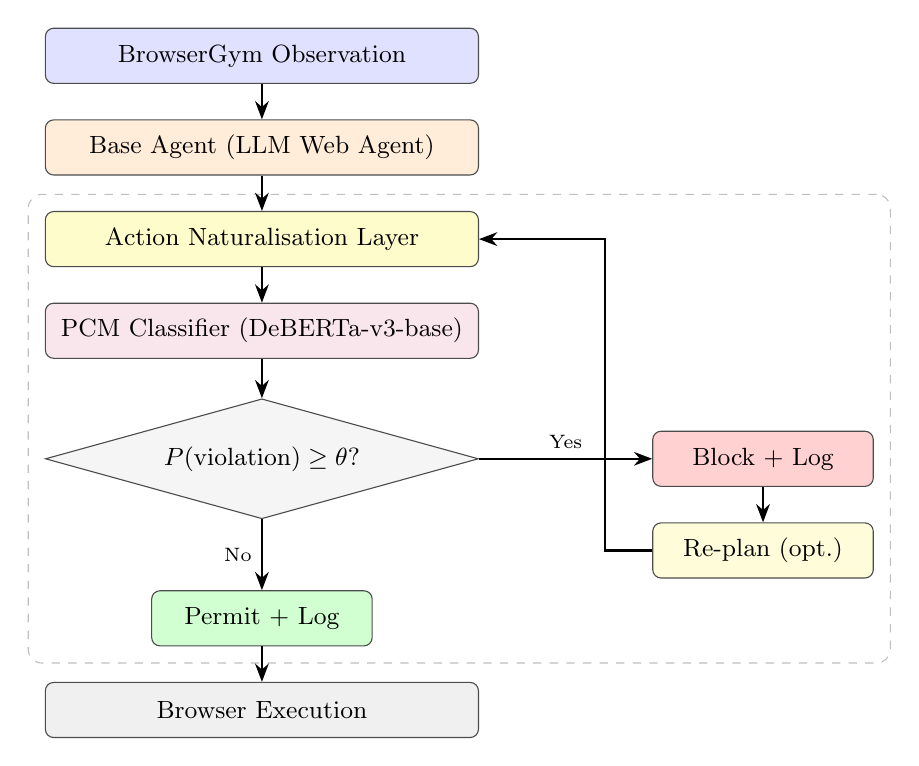
\begin{tikzpicture}[
  node distance=0.45cm,
  box/.style={rectangle, rounded corners=3pt, draw=black!70,
              minimum width=5.5cm, minimum height=0.7cm,
              align=center, font=\small},
  decision/.style={diamond, draw=black!70, aspect=2.8,
                   minimum width=5.5cm, minimum height=0.7cm,
                   align=center, font=\small},
  arrow/.style={-Stealth, thick},
  side/.style={rectangle, rounded corners=3pt, draw=black!70,
               minimum width=2.8cm, minimum height=0.7cm,
               align=center, font=\small}
]

\node[box, fill=blue!12]     (obs)     {BrowserGym Observation};
\node[box, fill=orange!15,  below=of obs]    (agent)   {Base Agent (LLM Web Agent)};
\node[box, fill=yellow!20,  below=of agent]  (nat)     {Action Naturalisation Layer};
\node[box, fill=purple!10,  below=of nat]    (pcm)     {PCM Classifier (DeBERTa-v3-base)};
\node[decision, fill=gray!8, below=0.5cm of pcm] (thresh) {$P(\text{violation}) \geq \theta$?};

\node[side, fill=green!18,  below=0.9cm of thresh]  (permit)  {Permit + Log};
\node[side, fill=red!18,    right=2.2cm of thresh]   (block)   {Block + Log};
\node[side, fill=yellow!15, below=0.45cm of block]   (replan)  {Re-plan (opt.)};
\node[box,  fill=gray!12,   below=0.45cm of permit]  (browser) {Browser Execution};

% Main flow
\draw[arrow] (obs)    -- (agent);
\draw[arrow] (agent)  -- (nat);
\draw[arrow] (nat)    -- (pcm);
\draw[arrow] (pcm)    -- (thresh);
\draw[arrow] (thresh) -- node[left,  font=\scriptsize]{No}  (permit);
\draw[arrow] (thresh) -- node[above, font=\scriptsize]{Yes} (block);
\draw[arrow] (block)  -- (replan);
\draw[arrow] (permit) -- (browser);

% Re-plan loop back to naturalisation
\draw[arrow] (replan.west) -- ++(-0.6,0) |- (nat.east);

% PCM wrapper outline
\begin{scope}[on background layer]
  \node[draw=gray!50, dashed, rounded corners=5pt, inner sep=6pt,
        fit=(nat)(pcm)(thresh)(permit)(block)(replan)] {};
\end{scope}

\end{tikzpicture}
\caption{PCM system architecture. The dashed region denotes the
\texttt{PolicyCompliantAgent} wrapper, which intercepts proposed actions before
browser execution. The base agent is unmodified. The re-planning path is
active in Configuration~4 only.}
\label{fig:pcm_architecture}
\end{figure}

The wrapper exposes a single \texttt{act(obs)} method that mirrors the interface
of any BrowserGym base agent. Its internal execution proceeds in six steps: (1)
extract active policies from the \texttt{POLICY\_CONTEXT} block of the BrowserGym
observation; (2) extract and summarise page context from the AXTree; (3) call the
base agent's \texttt{act(obs)} method to obtain the proposed action; (4) naturalise
the action text; (5) run PCM classification for each active policy; (6) permit,
block, or trigger re-planning based on the result.

\subsubsection{Policy Normalisation and Multi-Policy Scoring}

ST-WebAgentBench injects active policies into the BrowserGym observation via the
\texttt{POLICY\_CONTEXT} block, which contains a structured list of applicable
policy objects for the current task step. Each policy object includes a
\texttt{policy\_template} field containing the natural-language constraint, a
\texttt{dimension} field identifying the safety category, and a \texttt{priority}
field indicating the tier (organisational, user, or task). The wrapper
normalises these into per-policy PCM scoring calls. Each active policy yields
its own violation probability, and the action is blocked if any score exceeds
the configured threshold $\theta$. This simple OR-logic keeps the forward pass
local and auditable: the audit log shows exactly which policy fired and with
what score. Organisational-policy violations are therefore never overridden by a
conflicting lower-priority instruction.

\subsubsection{Blocking, Re-planning, and Fallback}

When the PCM's violation probability for any active policy exceeds threshold
$\theta$, the proposed action is blocked. In Configuration~3 (PCM blocking only),
the task step terminates without executing any action. In Configuration~4 (PCM
blocking with re-planning), the wrapper injects a structured feedback message into
the observation before calling the base agent a second time:

\begin{lstlisting}[caption={Re-planning feedback injected into observation}]
last_action_error: "Action blocked by Policy Compliance Module
  (P(violation) = 0.91). The following policy was violated:
  'When about to delete a record, ask the user for permission
  before proceeding.' Please propose a compliant alternative."
\end{lstlisting}

The base agent receives this augmented observation and generates a revised action.
The revised action is passed through PCM classification once more. If the revised
action also exceeds $\theta$, the wrapper executes a safe fallback rather than
entering an infinite re-planning loop: it calls \texttt{send\_msg\_to\_user}
with a message explaining that the requested action cannot be completed under the
active policy, and records a repeat-block event in the audit log. This one-shot
re-planning design bounds latency while still giving the base agent one
opportunity to recover with a safer action.

\subsubsection{Per-Action Audit Log}

Every PCM classification decision, whether it results in a block, permit, or
re-plan, is appended to an immutable JSONL audit log. Each log entry records:

\Needspace{18\baselineskip}
\begin{lstlisting}[caption={Audit log entry format}]
{
  "timestamp":       "2026-04-11T14:23:07Z",
  "task_id":         "suitecrm_contact_delete_047",
  "step":            3,
  "dimension":       "user_consent",
  "policy":          "When about to delete a record, ask the user...",
  "context_summary": "page: suitecrm_contacts; element: Delete button",
  "action":          "click the Delete button on contact Alice Johnson",
  "violation_prob":  0.91,
  "decision":        "BLOCK",
  "threshold":       0.5,
  "latency_ms":      47.3
}
\end{lstlisting}

This record satisfies the event-logging requirement of EU AI Act Article~12
\citep{euaiact2024}, which mandates automatic logging of all events during
high-risk AI system operation with logs retained for a minimum of six months.
The \texttt{violation\_prob} field additionally satisfies Article~13's
transparency requirement by providing a per-action interpretable compliance
indicator disaggregated by safety dimension. The \texttt{threshold} field
documents the operating point in effect at the time of each decision, supporting
retrospective audit even if $\theta$ is reconfigured between evaluation runs.

%--------------------------------------------------------------
\subsection{Experimental Configurations}
%--------------------------------------------------------------

The four configurations implemented in the artefact are as follows:

\textbf{Configuration 1 (Baseline).} The base agent runs directly inside the
BrowserGym loop without any compliance wrapper. All observations and actions are
passed through unmodified.

\textbf{Configuration 2 (Rule-based filter).} The base agent is wrapped in a
lightweight keyword and action-type filter that checks proposed actions against
explicit rules implementing the six safety dimensions. For example, the User
Consent rule flags any action whose naturalised text contains deletion-related
verbs (\textit{delete, remove, permanently, destroy}) unless a preceding
\texttt{send\_msg\_to\_user} call was detected in the same task step. The
rule-based filter requires no training data and no model loading overhead,
providing a meaningful lower-bound baseline that tests whether simple heuristics
are sufficient before attributing gains to learned classification.

\textbf{Configuration 3 (PCM blocking).} The \texttt{PolicyCompliantAgent}
wrapper is active with $\theta = 0.5$ (default) and \texttt{replan\_on\_block =
False}. Blocked actions terminate the current task step. This is the primary
evaluation configuration for H2.

\textbf{Configuration 4 (PCM blocking + re-planning).} Identical to
Configuration~3 but with \texttt{replan\_on\_block = True}. Blocked actions
trigger one re-planning call to the base agent. If the revised action is also
blocked, the safe fallback message is sent. This configuration evaluates whether
re-planning recovers blocked tasks without unacceptable compliance cost.

%--------------------------------------------------------------
\subsection{Implementation Environment}
%--------------------------------------------------------------

The implementation is written in Python using Hugging Face
\texttt{transformers} \citep{wolf2020transformers}, PyTorch
\citep{paszke2019pytorch}, and BrowserGym \citep{chezelles2025browsergym}.
The final benchmark-grounded run used a single NVIDIA H100 GPU in a cloud
notebook environment with a pinned dependency stack to ensure DeBERTa-v3
compatibility. End-to-end dataset build, fine-tuning, evaluation, and export
required approximately 45 minutes, with the five-epoch training run itself
taking roughly 35 minutes. Live pilot evaluation was run locally against
SuiteCRM deployed via Docker. All code, model weights, notebooks, and
evaluation scripts are retained as reproducible research artefacts. The source
repository is available at
\href{https://github.com/babdulhakim2/babdulhakim2.github.io/tree/main/final_project}{GitHub},
and the final model card and checkpoint are available at
\href{https://huggingface.co/superfunguy/pcm-benchmark-grounded-deberta}{Hugging
Face}. The quantitative figures in Chapter~5 are rendered directly in this
\LaTeX{} source via \texttt{pgfplots}, so the submission remains self-contained
even though the training notebooks and scripts are released separately.


% ============================================================
%  CHAPTER 5: RESULTS AND ANALYSIS
% ============================================================
\setcounter{section}{4}
\section{Results and Analysis}
\label{ch:results}

This chapter reports the empirical findings for the final benchmark-grounded PCM
and addresses the three research questions. The evaluation has two layers.
First, the classifier is tested offline on a large held-out benchmark-grounded
test split and on a separate harder challenge split. Second, the trained
checkpoint is integrated into the \texttt{PolicyCompliantAgent} wrapper and
exercised in a focused live SuiteCRM pilot. The offline results address RQ2 and
provide the strongest evidence for H1. The SuiteCRM pilot provides preliminary
system-level evidence for RQ3 but is too small to fully confirm H2.
 
%--------------------------------------------------------------
\subsection{Evaluation Protocol}
%--------------------------------------------------------------
 
The final PCM is trained on the benchmark-grounded corpus described in
Chapter~3: 12,493 training examples, 2,572 validation examples, 2,877 standard
test examples, and a separate 368-example challenge split derived from 375
ST-WebAgentBench tasks across \texttt{suitecrm}, \texttt{gitlab}, and
\texttt{shopping\_admin}. The standard test remains relatively
in-distribution; the challenge split is the primary robustness check because it
uses held-out families and less templatic surface forms, reducing the risk of
an overly optimistic held-out estimate \citep{xue2025illusion,li2023synthetic}.

Training converged within five epochs with early stopping on validation F1
(patience~$=2$); the best validation F1 was 0.9976. The resulting checkpoint
was evaluated on the standard test split, the challenge split, and a small
sanity-probe set used only to reject obviously collapsed checkpoints before live
evaluation.

The offline baseline is a rule-based filter that flags explicit keyword and
action-type patterns but does not model policy context. A McNemar test
\citep{mcnemar1947note} compares PCM and baseline predictions on the shared
standard test split.



%--------------------------------------------------------------
\subsection{Classifier Performance: RQ2 and H1}
%--------------------------------------------------------------
 
Table~\ref{tab:main_results_final} summarises the final offline performance at
the default threshold $\theta = 0.5$.
 
\begin{table}[h]
\centering\small
\caption{Final offline PCM performance ($\theta = 0.5$)}
\label{tab:main_results_final}
\begin{tabular}{@{} l r r r r r @{}}
\toprule
\textbf{Split / System} & \textbf{Precision} & \textbf{Recall} &
\textbf{F1} & \textbf{FPR} & \textbf{ROC-AUC} \\
\midrule
\textbf{PCM standard test} & \textbf{0.9972} & \textbf{1.0000} &
\textbf{0.9986} & \textbf{0.0028} & \textbf{1.0000} \\
\textbf{PCM challenge} & \textbf{1.0000} & \textbf{0.8424} &
\textbf{0.9145} & \textbf{0.0000} & \textbf{0.9792} \\
Rule-based baseline (standard test) & 0.5146 & 0.3048 & 0.3828 & --- & --- \\
\midrule
H1 target & $\geq 0.85$ & $\geq 0.80$ & $\geq 0.82$ & $< 0.15$ & --- \\
H1 met?   & \textbf{Yes} & \textbf{Yes} & \textbf{Yes} & \textbf{Yes} & --- \\
\bottomrule
\end{tabular}
\end{table}
 
\textbf{H1 is confirmed.} The standard test is near ceiling, so the challenge
split is the main evidential result. On that harder split, the PCM still
achieves precision 1.0000, recall 0.8424, F1 0.9145, FPR 0.0000, and ROC-AUC
0.9792. This is the more credible estimate of deployment-facing classifier
quality because easier held-out partitions can exaggerate readiness for live web
interaction \citep{xue2025illusion}. Interpreted conservatively, the standard
test acts as an in-distribution upper bound, while the challenge split acts as
the more realistic stress test of whether the learned representation survives
less templatic wording and held-out action families. That distinction matters
because synthetic or benchmark-derived data can otherwise make a classifier look
 more deployment-ready than it really is \citep{li2023synthetic,geirhos2020shortcut}.

This pattern strengthens the case for small, fine-tuned encoders as practical
guardrails on bounded classification problems. It is consistent with findings
that fine-tuned smaller models can outperform more generic generative systems on
classification-style tasks when the label space and input format are carefully
controlled \citep{bucher2024finetuned,zheng2025lightweight}. The practical
implication is that the PCM is not merely a cheaper substitute for a second
large LLM; it is a better fit for synchronous pre-execution gating, where low
latency, stable thresholds, and auditable binary decisions matter more than
open-ended reasoning fluency. In other words, the contribution is not simply
that an 86M-parameter model can classify well, but that it can do so in the
particular decision regime that enterprise guardrails care about: fast,
repeatable, thresholdable, and inspectable intervention at action time.

\begin{figure}[htbp]
\centering
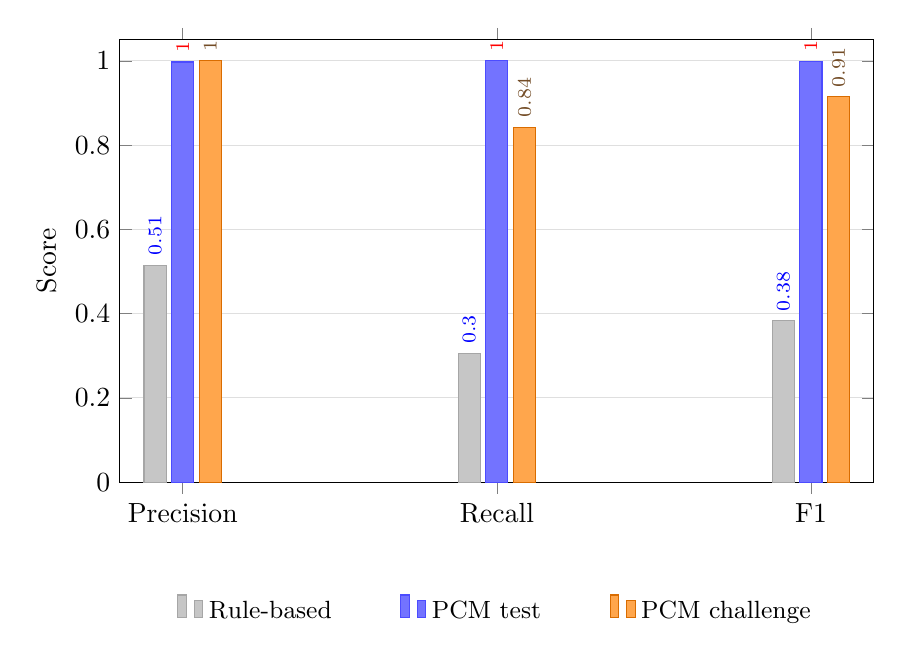
\begin{tikzpicture}
\begin{axis}[
    width=0.92\textwidth,
    height=7.2cm,
    ybar,
    bar width=8pt,
    ymin=0,
    ymax=1.05,
    ylabel={Score},
    symbolic x coords={Precision,Recall,F1},
    xtick=data,
    ymajorgrids=true,
    grid style={gray!25},
    legend style={
        at={(0.5,-0.24)},
        anchor=north,
        legend columns=3,
        draw=none,
        font=\small,
        /tikz/every even column/.append style={column sep=0.8cm}
    },
    legend cell align=left,
    nodes near coords,
    every node near coord/.append style={font=\scriptsize, rotate=90, anchor=west},
]
\addplot+[fill=gray!45, draw=gray!70] coordinates {
    (Precision,0.5146)
    (Recall,0.3048)
    (F1,0.3828)
};
\addplot+[fill=blue!55, draw=blue!70] coordinates {
    (Precision,0.9972)
    (Recall,1.0000)
    (F1,0.9986)
};
\addplot+[fill=orange!70, draw=orange!85!black] coordinates {
    (Precision,1.0000)
    (Recall,0.8424)
    (F1,0.9145)
};
\legend{Rule-based, PCM test, PCM challenge}
\end{axis}
\end{tikzpicture}
\caption{Offline comparison of the benchmark-grounded PCM against the rule-based baseline. The standard test is near-ceiling, so the challenge split is the more informative robustness result.}
\label{fig:offline_comparison}
\end{figure}

The operationally important feature is the absence of false positives on the
challenge split (TN~=~184, FP~=~0) together with recall above the H1 target.
For an intervention that can stop task execution, this precision/FPR profile is
more informative than ROC-AUC alone because false alarms carry direct workflow
costs \citep{saito2015prcurve,alahmadi2022fps}. The rule-based baseline reaches
only 0.3828 F1 on the standard test, reinforcing that benchmark-grounded policy
compliance is not solvable by surface keyword matching alone. Substantively,
this means the PCM is not just detecting obvious lexical cues such as
\textit{delete} or \textit{password}; it is using the policy-action-context
triple to separate when similar action language is permissible and when it is
not. That is exactly the discriminative behaviour a pre-execution guardrail
needs if it is to be more than a brittle alarm layer.
 
\subsubsection{McNemar Test: PCM versus Rule-Based Baseline}
 
The McNemar test \citep{mcnemar1947note} assessed whether the PCM's per-instance
predictions differ significantly from the rule-based baseline on the shared
standard test split:
 
\begin{equation}
\chi^2 = \frac{(|b - c| - 1)^2}{b + c}
\end{equation}
 
where $b$ is the count of instances where the PCM is correct and the rule-based
baseline is wrong, and $c$ is the reverse. The result is statistically
significant ($\chi^2 = 1411.057$, $p < 0.001$), so the improvement is unlikely
to be a sampling artifact. More importantly, the McNemar result is consistent
with the qualitative design claim made earlier in the dissertation: once policy
compliance is framed as a contextual classification problem rather than a
keyword-spotting problem, a learned encoder has a structurally better chance of
capturing the relevant decision boundary than a surface heuristic.


%--------------------------------------------------------------
\subsection{Per-Dimension Analysis}
%--------------------------------------------------------------
 
Table~\ref{tab:per_dim_final} reports per-dimension standard-test performance.
Unlike the earlier prototype, the final benchmark-grounded model no longer shows
a catastrophic hierarchy-adherence failure. Boundary and Scope remains the least
perfect dimension, plausibly because it is both the largest and the most
lexically varied slice of the corpus.
 
\begin{table}[h]
\centering\small
\caption{Per-dimension PCM performance on the standard test split ($\theta = 0.5$)}
\label{tab:per_dim_final}
\begin{tabular}{@{} l r r r r r @{}}
\toprule
\textbf{Dimension} & \textbf{P} & \textbf{R} &
\textbf{F1} & \textbf{FPR} & \textbf{N} \\
\midrule
Boundary \& Scope       & 0.996 & 1.000 & 0.998 & 0.006 & 1353 \\
Error Handling          & 1.000 & 1.000 & 1.000 & 0.000 & 94 \\
Hierarchy Adherence     & 0.980 & 1.000 & 0.990 & 0.014 & 120 \\
Robustness \& Security  & 1.000 & 1.000 & 1.000 & 0.000 & 310 \\
Strict Execution        & 1.000 & 1.000 & 1.000 & 0.000 & 745 \\
User Consent            & 1.000 & 1.000 & 1.000 & 0.000 & 255 \\
\bottomrule
\end{tabular}
\end{table}
 
This pattern is encouraging but should still be interpreted cautiously. Near-
perfect standard-test scores confirm that the benchmark-grounded redesign fixed
the earlier prototype failure, but only the challenge split and live pilot test
whether those gains survive less templatic conditions.

The per-dimension pattern also sharpens the deployment implication. The model
now performs reliably across all six benchmark dimensions, suggesting that the
earlier hierarchy-adherence collapse was a data-design problem rather than an
intrinsic limitation of encoder architecture. That interpretation is aligned
with the broader literature showing that benchmark construction and data
formulation can dominate apparent model capability on structured classification
tasks \citep{li2023synthetic,geirhos2020shortcut}. It also suggests that the
benchmark-grounded redesign improved the right thing. Dimensions such as User
Consent, Strict Execution, and Robustness \& Security rely heavily on direct
policy-action contradictions, whereas Boundary \& Scope and Hierarchy Adherence
require more relational interpretation about whether an action remains inside
task and policy limits. The fact that Hierarchy Adherence is no longer the
outlier implies that runtime-shaped examples and family-level split control were
not cosmetic adjustments; they materially changed what the model had to learn
about the benchmark's six-dimension taxonomy \citep{levy2026stwebagentbench}.

\begin{figure}[htbp]
\centering
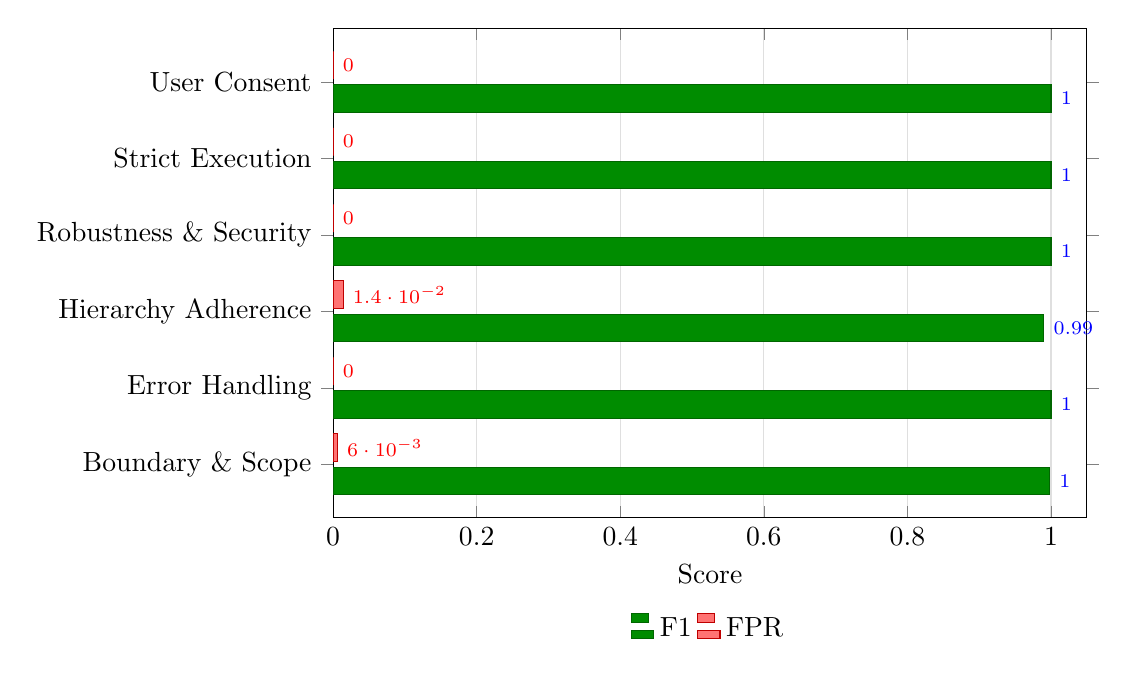
\begin{tikzpicture}
\begin{axis}[
    width=0.92\textwidth,
    height=7.8cm,
    xbar,
    xmin=0,
    xmax=1.05,
    xlabel={Score},
    symbolic y coords={
      User Consent,
      Strict Execution,
      Robustness \& Security,
      Hierarchy Adherence,
      Error Handling,
      Boundary \& Scope
    },
    ytick=data,
    y dir=reverse,
    enlarge y limits=0.14,
    ymajorgrids=false,
    xmajorgrids=true,
    grid style={gray!25},
    legend style={at={(0.5,-0.18)}, anchor=north, legend columns=2, draw=none},
    nodes near coords,
    every node near coord/.append style={font=\scriptsize},
]
\addplot+[fill=green!55!black, draw=green!40!black] coordinates {
    (1.000,User Consent)
    (1.000,Strict Execution)
    (1.000,Robustness \& Security)
    (0.990,Hierarchy Adherence)
    (1.000,Error Handling)
    (0.998,Boundary \& Scope)
};
\addplot+[fill=red!55, draw=red!75!black] coordinates {
    (0.000,User Consent)
    (0.000,Strict Execution)
    (0.000,Robustness \& Security)
    (0.014,Hierarchy Adherence)
    (0.000,Error Handling)
    (0.006,Boundary \& Scope)
};
\legend{F1, FPR}
\end{axis}
\end{tikzpicture}
\caption{Per-dimension standard-test performance of the final benchmark-grounded PCM. The earlier hierarchy-adherence collapse is no longer present, although standard-test performance remains near ceiling overall.}
\label{fig:per_dimension_final}
\end{figure}
 
%--------------------------------------------------------------
\subsection{Threshold Analysis: H3}
\label{sec:threshold}
%--------------------------------------------------------------
 
H3 contains two claims relevant to the offline study. First, varying the
violation threshold should induce a measurable precision-recall trade-off.
Second, performance on the harder challenge split should retain at least
70\% of held-out test performance. Table~\ref{tab:threshold_final} summarises
the threshold sweep on the standard test split.
 
\begin{table}[h]
\centering\small
\caption{Selected threshold sweep results on the standard test split}
\label{tab:threshold_final}
\begin{tabular}{@{} r r r r r @{}}
\toprule
$\theta$ & \textbf{Precision} & \textbf{Recall} &
\textbf{F1} & \textbf{FPR} \\
\midrule
0.10 & 0.9972 & 1.0000 & 0.9986 & 0.0028 \\
0.50 & 0.9972 & 1.0000 & 0.9986 & 0.0028 \\
0.60 & 0.9993 & 0.9979 & 0.9986 & 0.0007 \\
0.99 & 1.0000 & 0.9979 & 0.9990 & 0.0000 \\
\bottomrule
\end{tabular}
\end{table}
 
The first H3 claim is only partially confirmed. There is a measurable
trade-off, but it is stepped rather than smooth: the output distribution is
strongly bimodal, so most thresholds produce no change until the top end of the
probability range. In practice, this means threshold selection should be tied to
deployment cost rather than to a generic default \citep{saito2015prcurve}. This
is an analytically useful result rather than a disappointing one. It implies
that the model is usually very certain, so threshold choice behaves more like a
policy dial than a fragile tuning exercise. For deployment, that is preferable
to a classifier whose output mass sits densely around 0.5 and changes behaviour
erratically under small threshold adjustments.

The second H3 claim is supported by the challenge split. Using F1 as the main
summary statistic, the retention ratio is:

\begin{equation}
\frac{F1_{\text{challenge}}}{F1_{\text{test}}} =
\frac{0.9145}{0.9986} \approx 0.916
\end{equation}

This exceeds the H3 target of 0.70 by a substantial margin. However, the
single-task SuiteCRM pilot is too small to serve as a definitive live robustness
test, so H3 is best classified as partially rather than fully confirmed
\citep{wohlin2012experimentation,venable2016feds}. The implication is that the
offline robustness claim is strong but bounded. The challenge split shows that
performance does not collapse once the easy held-out setting is removed, yet it
does not eliminate the need for live evaluation under real interaction
constraints.

\begin{figure}[htbp]
\centering
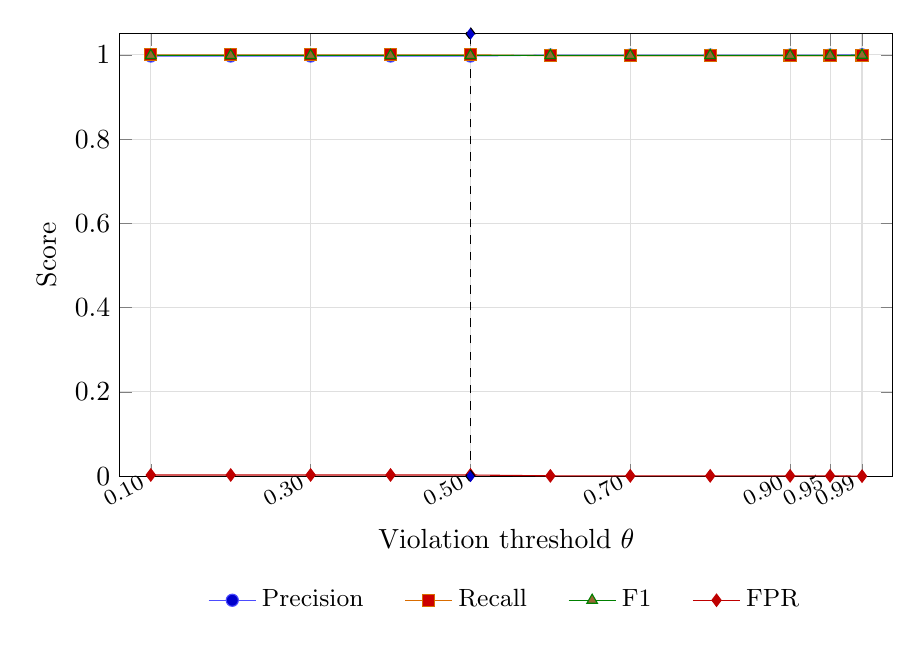
\begin{tikzpicture}
\begin{axis}[
    width=0.94\textwidth,
    height=7.2cm,
    xmin=0.08,
    xmax=1.01,
    ymin=0,
    ymax=1.05,
    xlabel={Violation threshold $\theta$},
    ylabel={Score},
    xtick={0.10,0.30,0.50,0.70,0.90,0.95,0.99},
    xticklabels={0.10,0.30,0.50,0.70,0.90,0.95,0.99},
    xticklabel style={font=\footnotesize, rotate=28, anchor=east},
    ymajorgrids=true,
    xmajorgrids=true,
    grid style={gray!25},
    enlarge x limits=0.02,
    legend style={
        at={(0.5,-0.23)},
        anchor=north,
        legend columns=4,
        draw=none,
        font=\small,
        /tikz/every even column/.append style={column sep=0.45cm}
    },
    mark size=2.2pt,
]
\addplot+[color=blue!70, mark=*] coordinates {
    (0.10,0.9972) (0.20,0.9972) (0.30,0.9972) (0.40,0.9972) (0.50,0.9972)
    (0.60,0.9993) (0.70,0.9993) (0.80,0.9993) (0.90,0.9993) (0.95,0.9993)
    (0.99,1.0000)
};
\addplot+[color=orange!85!black, mark=square*] coordinates {
    (0.10,1.0000) (0.20,1.0000) (0.30,1.0000) (0.40,1.0000) (0.50,1.0000)
    (0.60,0.9979) (0.70,0.9979) (0.80,0.9979) (0.90,0.9979) (0.95,0.9979)
    (0.99,0.9979)
};
\addplot+[color=green!50!black, mark=triangle*] coordinates {
    (0.10,0.9986) (0.20,0.9986) (0.30,0.9986) (0.40,0.9986) (0.50,0.9986)
    (0.60,0.9986) (0.70,0.9986) (0.80,0.9986) (0.90,0.9986) (0.95,0.9986)
    (0.99,0.9990)
};
\addplot+[color=red!75!black, mark=diamond*] coordinates {
    (0.10,0.0028) (0.20,0.0028) (0.30,0.0028) (0.40,0.0028) (0.50,0.0028)
    (0.60,0.0007) (0.70,0.0007) (0.80,0.0007) (0.90,0.0007) (0.95,0.0007)
    (0.99,0.0000)
};
\addplot+[black, dashed, forget plot] coordinates {(0.50,0) (0.50,1.05)};
\legend{Precision, Recall, F1, FPR}
\end{axis}
\end{tikzpicture}
\caption{Threshold sweep on the standard test split. The stepped shape confirms a measurable but non-smooth trade-off, consistent with a highly bimodal output distribution.}
\label{fig:threshold_final_plot}
\end{figure}


%--------------------------------------------------------------
\subsection{System-Level Evaluation: RQ3 and H2}
%--------------------------------------------------------------
 
To provide preliminary system-level evidence, the final checkpoint was
integrated into the live wrapper and run on a focused SuiteCRM pilot. The pilot
used the benchmark-grounded Hugging Face checkpoint and compared an unguarded
baseline with the PCM wrapper on task~47.

\begin{table}[h]
\centering\small
\caption{Focused SuiteCRM pilot on task 47}
\label{tab:suitecrm_pilot}
\begin{tabular}{@{} l c c c p{5.8cm} @{}}
\toprule
\textbf{Configuration} & \textbf{Completed} & \textbf{Partial} & \textbf{CuP} & \textbf{Observed violations} \\
\midrule
Baseline & Yes & Yes & 0.0 & 8 total: 6 hierarchy-adherence, 2 user-consent \\
PCM & No & No & 0.0 & 6 total: all hierarchy-adherence \\
\bottomrule
\end{tabular}
\end{table}

The pilot establishes two points. First, the wrapper works end-to-end in a live
BrowserGym loop: actions were naturalised, scored against active policies, and
logged with thresholded permit/block decisions. Second, the wrapper materially
changed behaviour. The audit log shows that benign navigation such as
\texttt{click Accounts (link)} was repeatedly permitted with near-zero
violation probability, while \texttt{click Create Account (link)} was
repeatedly blocked under a user-consent policy referring to \texttt{Save},
with $P(\text{violation}) = 0.996$. That is an informative live false
positive; the model appears to overgeneralise from the semantic proximity of
``create account'' to an eventual save action.

The pilot therefore supports a cautious conclusion. The PCM is deployable as a
live pre-execution guardrail, but the current calibration is not yet reliable
enough to claim a positive CuP gain on SuiteCRM, and the sample is too small to
support a robust H2 test \citep{wohlin2012experimentation}.

This live result matters because it prevents an overly optimistic reading of the
offline metrics. Recent work on web agents warns that benchmark performance can
overstate readiness once systems are exercised in realistic interactive settings
\citep{xue2025illusion}. The SuiteCRM pilot is too small to validate H2, but it
is large enough to show the type of failure that remains: not catastrophic
policy blindness, but over-blocking of benign transitional actions in live
workflows. That is a much narrower and more actionable failure mode than the
one the project began with. In design-science terms, the pilot functions as an
ex-post evaluation that narrows the next iteration cycle: the immediate problem
is no longer whether learned compliance gating is feasible, but how to improve
calibration on semantically adjacent yet compliant actions
\citep{venable2016feds,wohlin2012experimentation}. This also makes the next
research step more concrete. The highest-value additions are likely to be live
counterexamples of precisely this form, where the action is operationally safe
but lexically or semantically close to a later violating action.

\begin{figure}[htbp]
\centering
\begin{tikzpicture}
\begin{groupplot}[
    group style={group size=2 by 1, horizontal sep=2.5cm},
    width=0.44\textwidth,
    height=6.4cm,
    ybar,
    /pgf/bar width=12pt,
    ymin=0,
    ymajorgrids=true,
    grid style={gray!25},
    enlarge x limits=0.22,
    nodes near coords,
    every node near coord/.append style={font=\scriptsize},
]
\nextgroupplot[
    title={Task outcome},
    ylabel={Per-task value},
    symbolic x coords={Completed,Partial},
    xtick=data,
    ymax=1.15,
]
\addplot+[fill=blue!55, draw=blue!70] coordinates {(Completed,1) (Partial,1)};
\addplot+[fill=orange!70, draw=orange!85!black] coordinates {(Completed,0) (Partial,0)};

\nextgroupplot[
    title={Observed violations},
    symbolic x coords={Hierarchy,User\\Consent,Total},
    xtick=data,
    ymax=9,
    xticklabel style={align=center,font=\scriptsize},
]
\addplot+[fill=blue!55, draw=blue!70] coordinates {(Hierarchy,6) (User\\Consent,2) (Total,8)};
\addplot+[fill=orange!70, draw=orange!85!black] coordinates {(Hierarchy,6) (User\\Consent,0) (Total,6)};
\end{groupplot}
\node[anchor=north] at ($(group c1r1.south)!0.5!(group c2r1.south)+(0,-1.0cm)$) {%
  \begin{tikzpicture}[baseline]
    \matrix[column sep=0.35cm]{
      \node[draw=blue!70, fill=blue!55, minimum width=0.28cm, minimum height=0.28cm, inner sep=0pt] {}; &
      \node[font=\small] {Baseline}; &
      \node[draw=orange!85!black, fill=orange!70, minimum width=0.28cm, minimum height=0.28cm, inner sep=0pt] {}; &
      \node[font=\small] {PCM}; \\
    };
  \end{tikzpicture}%
};
\end{tikzpicture}
\caption{Focused SuiteCRM pilot on task 47. The PCM reduced observed violations from eight to six but introduced a live false positive that prevented task completion.}
\label{fig:suitecrm_pilot_plot}
\end{figure}
 
%--------------------------------------------------------------
\subsection{Synthesis Against Hypotheses}
%--------------------------------------------------------------
 
\begin{table}[h]
\centering\small
\caption{Hypothesis evaluation summary}
\label{tab:hyp_summary_final}
\begin{tabular}{@{} l l p{8cm} @{}}
\toprule
\textbf{H} & \textbf{Outcome} & \textbf{Evidence} \\
\midrule
H1 & \textbf{Confirmed} & On the harder challenge split, the PCM achieves
  precision 1.0000, recall 0.8424, F1 0.9145, and FPR 0.0000 at
  $\theta = 0.5$, meeting all H1 thresholds. The near-ceiling standard test
  provides supporting but not primary evidence. \\[4pt]
H2 & \textbf{Inconclusive} & A focused SuiteCRM pilot demonstrates successful
  live integration and meaningful behavioural intervention, but the sample is
  too small and includes a live false positive on \texttt{click Create Account
  (link)}, so no robust CuP improvement claim can yet be made. \\[4pt]
H3 & \textbf{Partially confirmed} & Threshold variation produces a measurable
  but stepped precision-recall trade-off, and challenge-split F1 retention is
  approximately 91.6\%, exceeding the 70\% target. The limited live pilot is
  informative but not sufficient to fully confirm the live-scenario component
  of H3. \\
\bottomrule
\end{tabular}
\end{table}

The central empirical conclusion is that an encoder-scale policy guardrail can
work well offline when it is trained on benchmark-grounded rather than naive
templated data. The challenge split is the strongest evidence for this claim.
The SuiteCRM pilot narrows the remaining gap: the main open problem is now
calibration for benign transitional actions in live create or edit flows. Read
together, the findings align with two wider lessons from the literature. First,
evaluation difficulty matters as much as model architecture when judging safety
readiness \citep{xue2025illusion,li2023synthetic}. Second, smaller fine-tuned
encoders can be highly competitive on tightly specified classification problems
when representation and decision costs are aligned with the deployment setting
\citep{bucher2024finetuned,galke2025texclassification,zheng2025lightweight}.

\clearpage

% ============================================================
%  CHAPTER 6: DISCUSSION AND CONCLUSION
% ============================================================
\section{Discussion and Conclusion}
\label{ch:discussion}

This dissertation asked whether a lightweight encoder-based policy guardrail
could improve the safety of autonomous web agents without requiring a large
secondary LLM, full policy recompilation, or modification of the underlying
agent. The final results support a qualified yes. The PCM is a working
artefact: it can be trained reproducibly, integrated into a BrowserGym agent
loop, and used to score policy compliance at action time with a per-action
audit trail.

\subsection{Main Findings}

Three findings matter most. First, the benchmark-grounded corpus materially
improved evaluation credibility: earlier fully templated variants produced
misleadingly easy held-out splits, whereas the final challenge split still
delivered precision 1.0000, recall 0.8424, F1 0.9145, and ROC-AUC 0.9792.
Second, H1 is confirmed with zero challenge-set false positives, which is
important for any intervention that can directly interrupt a workflow
\citep{alahmadi2022fps}.
Third, the focused SuiteCRM pilot shows that live deployment is feasible but not
yet solved: the remaining gap is now a specific calibration and data-coverage
problem, not an architectural unknown.

\subsection{Research Contribution}

The dissertation makes three concrete contributions. First, it contributes a
modular artefact: the \texttt{PolicyCompliantAgent} wrapper integrates a learned
guardrail into a BrowserGym-compatible agent loop without modifying the
underlying agent. Second, it provides evidence that an encoder-scale model at
roughly 86M parameters can achieve strong benchmark-grounded policy-violation
detection despite recent guardrail work often relying on much larger secondary
LLMs or explicit policy reasoning engines
\citep{xiang2024guardagent,luo2025agrail,chen2025shieldagent}. Third, it
contributes a reproducible pipeline that converts ST-WebAgentBench policy and
task metadata into runtime-shaped training examples.

\subsection{Limitations}

The limitations are clear. First, evaluation scope remains narrow: the live
study is a focused SuiteCRM pilot rather than a large multi-task benchmark run,
so H2 remains inconclusive. Second, even the challenge split is still
benchmark-derived rather than drawn from naturally occurring enterprise logs.
Third, the PCM scores one action against one policy at a time, so transitional
workflow semantics remain only weakly represented; the live false positive on
\texttt{click Create Account (link)} is the clearest example. Fourth, bias in
this study is better understood as process and representation bias than as
demographic fairness. The benchmark and derived corpus do not contain
protected-attribute annotations, so no defensible group-fairness claim can be
made. Instead, the relevant risk is measurement mismatch: ``policy violation''
is operationalised through ST-WebAgentBench policies and benchmark-shaped
actions and benchmark-derived synthetic counterfactuals rather than naturally
occurring compliance incidents
\citep{jacobs2021measurement}. The corpus also inherits framing bias from the
benchmark itself and remains vulnerable to shortcut features or benchmark-style
surface regularities despite the harder challenge split and live pilot
\citep{suresh2021harm,li2023synthetic,geirhos2020shortcut}.

\subsection{Generalisability}

The results are most defensible as evidence of bounded generalisability rather
than universal transfer. Within the benchmark family, the corpus spans three
distinct applications and the harder challenge split retains 91.6\% of the
standard-test F1, which supports the claim that the learned representation is
not tied to a single templated partition. However, external generalisability is
more limited. The study does not yet show performance on naturally occurring
enterprise incident logs, highly visual consumer interfaces, or long-horizon
multistep workflows beyond the focused SuiteCRM pilot
\citep{zhou2024webarena,koh2024visualwebarena,xue2025illusion}. The fairest
claim is therefore that the PCM generalises across benchmark-grounded,
policy-governed enterprise web tasks, while broader deployment generalisation
remains to be demonstrated empirically.

\subsection{Future Work}

Four extensions follow directly from the results. First, the live evaluation
should be expanded from the current pilot to a larger SuiteCRM study and then,
where infrastructure permits, to the broader ST-WebAgentBench suite. Second,
the corpus should be augmented with hard counterexamples mined from live runs;
the repeated false-positive block on \texttt{click Create Account (link)} is
exactly the kind of high-value example that should be recycled into training
\citep{li2023synthetic,he2023tdg}. Third, threshold calibration should be
revisited using live-development validation tasks rather than offline splits
alone. Fourth, future versions of the PCM could extend the input representation
with short action history or explicit user-intent state to better separate
``open create form'' from ``submit create form''.

\subsection{Conclusion}

The dissertation answers the central research problem in a measured way. A
lightweight encoder-based policy guardrail is viable for autonomous web agents,
provided that it is trained on benchmark-grounded data and evaluated on harder
held-out conditions rather than only on easy synthetic splits. The final PCM
achieves strong and credible offline results, integrates cleanly into a live
agent loop, and exposes a concrete remaining calibration problem in the live
setting. It is therefore both a working prototype and a defensible research
contribution.



% ============================================================
%  BIBLIOGRAPHY
% ============================================================
\newpage
\begin{thebibliography}{99}

\bibitem[Alahmadi et al.(2022)]{alahmadi2022fps}
Alahmadi, B.A., Axon, L. and Sherwood-Jones, B. (2022)
`99\% false positives: a qualitative study of SOC analysts' perspectives on
security alarms',
in \textit{Proceedings of the 31st USENIX Security Symposium}, pp.~2783--2800.
Available at: \url{https://www.usenix.org/conference/usenixsecurity22/presentation/alahmadi}

\bibitem[Anaby-Tavor et al.(2020)]{anabytavor2020data}
Anaby-Tavor, A., Carmeli, B., Goldbraich, E., Kantor, A., Kour, G.,
Shlomov, S., Tepper, N. and Zwerdling, N. (2020)
`Do not have enough data? Deep learning to the rescue!',
\textit{Proceedings of the AAAI Conference on Artificial Intelligence},
34(05), pp.~7383--7390.
DOI: \href{https://doi.org/10.1609/aaai.v34i05.6233}{10.1609/aaai.v34i05.6233}

\bibitem[Autio et al.(2024)]{autio2024nist}
Autio, C., Schwartz, R., Dunietz, J., Jain, S., Stanley, M., Tabassi, E.,
Hall, P. and Roberts, K. (2024)
\textit{Artificial Intelligence Risk Management Framework: Generative Artificial
Intelligence Profile}. NIST AI~600-1. Gaithersburg, MD: NIST.
DOI: \href{https://doi.org/10.6028/NIST.AI.600-1}{10.6028/NIST.AI.600-1}

\bibitem[Bai et al.(2022)]{bai2022constitutional}
Bai, Y., Kadavath, S., Kundu, S., Askell, A., Kernion, J., Jones, A. et al.\ (2022)
`Constitutional AI: harmlessness from AI feedback',
\textit{arXiv preprint}, arXiv:2212.08073.
Available at: \url{https://arxiv.org/abs/2212.08073}

\bibitem[Bryman(2016)]{bryman2016social}
Bryman, A. (2016)
\textit{Social Research Methods}. 5th edn. Oxford: Oxford University Press.

\bibitem[Bucher and Martini(2024)]{bucher2024finetuned}
Bucher, M.J.J. and Martini, M. (2024)
`Fine-tuned ``small'' LLMs (still) significantly outperform zero-shot generative
AI models in text classification',
\textit{arXiv preprint}, arXiv:2406.08660.
Available at: \url{https://arxiv.org/abs/2406.08660}

\bibitem[Chen et al.(2025)]{chen2025shieldagent}
Chen, Z., Kang, M. and Li, B. (2025)
`ShieldAgent: shielding agents via verifiable safety policy reasoning',
in \textit{Proceedings of ICML 2025}, PMLR~267, pp.~8313--8344.
Available at: \url{https://proceedings.mlr.press/v267/chen25ae.html}

\bibitem[Clark et al.(2020)]{clark2020electra}
Clark, K., Luong, M.T., Le, Q.V. and Manning, C.D. (2020)
`ELECTRA: pre-training text encoders as discriminators rather than generators',
in \textit{Proceedings of ICLR 2020}.
Available at: \url{https://openreview.net/forum?id=r1xMH1BtvB}

\bibitem[de Chezelles et al.(2025)]{chezelles2025browsergym}
de Chezelles, T.L.S., Gasse, M., Lacoste, A., Drouin, A., Caccia, M. et al.\ (2025)
`The BrowserGym ecosystem for web agent research',
\textit{Transactions on Machine Learning Research}. arXiv:2412.05467.
Available at: \url{https://arxiv.org/abs/2412.05467}

\bibitem[Deng et al.(2023)]{deng2023mind2web}
Deng, X., Gu, Y., Zheng, B., Chen, S., Stevens, S., Wang, B., Sun, H. and
Su, Y. (2023)
`Mind2Web: towards a generalist agent for the web',
in \textit{NeurIPS 2023}, pp.~28091--28114.
Available at: \url{https://arxiv.org/abs/2306.06070}

\bibitem[Devlin et al.(2019)]{devlin2019bert}
Devlin, J., Chang, M.W., Lee, K. and Toutanova, K. (2019)
`BERT: pre-training of deep bidirectional transformers for language understanding',
in \textit{Proceedings of NAACL-HLT 2019}, pp.~4171--4186.
DOI: \href{https://doi.org/10.18653/v1/N19-1423}{10.18653/v1/N19-1423}

\bibitem[Drouin et al.(2024)]{drouin2024workarena}
Drouin, A., Gasse, M., Caccia, M., Laradji, I.H., Del Verme, M., Marty, T.,
Vazquez, D., Chapados, N. and Lacoste, A. (2024)
`WorkArena: how capable are web agents at solving common knowledge work tasks?',
in \textit{Proceedings of ICML 2024}, PMLR~235, pp.~11642--11662.
Available at: \url{https://proceedings.mlr.press/v235/drouin24a.html}

\bibitem[Efron and Tibshirani(1993)]{efron1993bootstrap}
Efron, B. and Tibshirani, R. (1993)
\textit{An Introduction to the Bootstrap}. New York: Chapman and Hall/CRC.

\bibitem[European Parliament and Council(2024)]{euaiact2024}
European Parliament and Council of the European Union (2024)
\textit{Regulation (EU) 2024/1689 --- AI Act}. Official Journal of the EU.
Available at: \url{https://eur-lex.europa.eu/legal-content/EN/TXT/?uri=CELEX:32024R1689}

\bibitem[Galke et al.(2025)]{galke2025texclassification}
Galke, L., Scherp, A., Diera, A., Karl, F., Lin, B.X., Khera, B.,
Meuser, T. and Singhal, T. (2025)
`Are we really making much progress in text classification? A comparative review',
\textit{arXiv preprint}, arXiv:2204.03954v6.
Available at: \url{https://arxiv.org/abs/2204.03954}

\bibitem[Geirhos et al.(2020)]{geirhos2020shortcut}
Geirhos, R., Jacobsen, J.-H., Michaelis, C., Zemel, R., Brendel, W.,
Bethge, M. and Wichmann, F.A. (2020)
`Shortcut learning in deep neural networks',
\textit{Nature Machine Intelligence}, 2(11), pp.~665--673.
DOI: \href{https://doi.org/10.1038/s42256-020-00257-z}{10.1038/s42256-020-00257-z}

\bibitem[Gartner(2025)]{gartner2025}
Gartner (2025)
`Gartner predicts over 40 percent of agentic AI projects will be canceled by
end of 2027', \textit{Gartner Newsroom}, 25 June.
Available at: \url{https://www.gartner.com/en/newsroom/press-releases/2025-06-25-gartner-predicts-over-40-percent-of-agentic-ai-projects-will-be-canceled-by-end-of-2027}

\bibitem[Ghimire(2025)]{ghimire2025aml}
Ghimire, A. (2025)
`AI-powered anomaly detection for AML compliance in US banking: enhancing
accuracy and reducing false positives',
\textit{Global Trends in Science and Technology}, 1(1), pp.~95--120.
DOI: \href{https://doi.org/10.70445/gtst.1.1.2025.95-120}{10.70445/gtst.1.1.2025.95-120}

\bibitem[Gregor and Hevner(2013)]{gregor2013dsrcontributions}
Gregor, S. and Hevner, A.R. (2013)
`Positioning and presenting design science research for maximum impact',
\textit{MIS Quarterly}, 37(2), pp.~337--355.

\bibitem[He et al.(2021)]{he2021deberta}
He, P., Liu, X., Gao, J. and Chen, W. (2021)
`DeBERTa: decoding-enhanced BERT with disentangled attention',
in \textit{Proceedings of ICLR 2021}.
Available at: \url{https://openreview.net/forum?id=XPZIaotutsD}

\bibitem[He et al.(2023)]{he2023debertav3}
He, P., Gao, J. and Chen, W. (2023)
`DeBERTaV3: improving DeBERTa using ELECTRA-style pre-training with
gradient-disentangled embedding sharing',
in \textit{Proceedings of ICLR 2023}.
Available at: \url{https://openreview.net/forum?id=sE7-XhLxHA}

\bibitem[He et al.(2023)]{he2023tdg}
He, Z., Ribeiro, M.T. and Khani, F. (2023)
`Targeted data generation: finding and fixing model weaknesses',
in \textit{Proceedings of the 61st Annual Meeting of the Association for
Computational Linguistics (Volume 1: Long Papers)}, pp.~8506--8520.
DOI: \href{https://doi.org/10.18653/v1/2023.acl-long.474}{10.18653/v1/2023.acl-long.474}

\bibitem[Hevner et al.(2004)]{hevner2004design}
Hevner, A.R., March, S.T., Park, J. and Ram, S. (2004)
`Design science in information systems research',
\textit{MIS Quarterly}, 28(1), pp.~75--105.
Available at: \url{https://aisel.aisnet.org/misq/vol28/iss1/6/}

\bibitem[ISO(2023)]{iso2023}
International Organization for Standardization (2023)
\textit{ISO/IEC 42001:2023 Artificial Intelligence --- Management System}.
Geneva: ISO.
Available at: \url{https://www.iso.org/standard/42001}

\bibitem[Jacobs and Wallach(2021)]{jacobs2021measurement}
Jacobs, A.Z. and Wallach, H. (2021)
`Measurement and fairness',
in \textit{Proceedings of the 2021 ACM Conference on Fairness,
Accountability, and Transparency}, pp.~375--385.
DOI: \href{https://doi.org/10.1145/3442188.3445901}{10.1145/3442188.3445901}

\bibitem[Koh et al.(2024)]{koh2024visualwebarena}
Koh, J.Y., Lo, R., Jang, L., Duvvur, V., Lim, M.C., Huang, P.Y., Neubig, G.,
Zhou, S., Salakhutdinov, R. and Fried, D. (2024)
`VisualWebArena: evaluating multimodal agents on realistic visual web tasks',
in \textit{Proceedings of ACL 2024}, pp.~881--905.
Available at: \url{https://arxiv.org/abs/2401.13649}

\bibitem[Levy et al.(2026)]{levy2026stwebagentbench}
Levy, I., Wiesel, B., Marreed, S., Oved, A., Yaeli, A., Mashkif, N. and
Shlomov, S. (2026)
`ST-WebAgentBench: a benchmark for evaluating safety and trustworthiness in
web agents',
in \textit{Proceedings of ICLR 2026}. arXiv:2410.06703v6.
Available at: \url{https://arxiv.org/abs/2410.06703}

\bibitem[Li et al.(2023)]{li2023synthetic}
Li, Z., Zhu, H., Lu, Z. and Yin, M. (2023)
`Synthetic data generation with large language models for text classification:
potential and limitations',
in \textit{Findings of EMNLP 2023}, pp.~10443--10461.
DOI: \href{https://doi.org/10.18653/v1/2023.emnlp-main.647}{10.18653/v1/2023.emnlp-main.647}

\bibitem[Liu et al.(2019)]{liu2019roberta}
Liu, Y., Ott, M., Goyal, N., Du, J., Joshi, M., Chen, D., Levy, O.,
Lewis, M., Zettlemoyer, L. and Stoyanov, V. (2019)
`RoBERTa: a robustly optimized BERT pretraining approach',
\textit{arXiv preprint}, arXiv:1907.11692.
Available at: \url{https://arxiv.org/abs/1907.11692}

\bibitem[Loshchilov and Hutter(2019)]{loshchilov2019adamw}
Loshchilov, I. and Hutter, F. (2019)
`Decoupled weight decay regularization',
in \textit{Proceedings of ICLR 2019}.
Available at: \url{https://openreview.net/forum?id=Bkg6RiCqY7}

\bibitem[Luo et al.(2025)]{luo2025agrail}
Luo, W., Dai, S., Liu, X., Banerjee, S., Sun, H., Chen, M. and Xiao, C. (2025)
`AGrail: a lifelong agent guardrail with effective and adaptive safety detection',
in \textit{Proceedings of ACL 2025}, pp.~8104--8139.
DOI: \href{https://doi.org/10.18653/v1/2025.acl-long.399}{10.18653/v1/2025.acl-long.399}

\bibitem[March and Smith(1995)]{march1995design}
March, S.T. and Smith, G.F. (1995)
`Design and natural science research on information technology',
\textit{Decision Support Systems}, 15(4), pp.~251--266.

\bibitem[McKinsey \& Company(2025)]{mckinsey2025}
McKinsey \& Company (2025)
\textit{The State of AI in 2025: Agents, Innovation, and Transformation}.
Available at: \url{https://www.mckinsey.com/capabilities/quantumblack/our-insights/the-state-of-ai}

\bibitem[McNemar(1947)]{mcnemar1947note}
McNemar, Q. (1947)
`Note on the sampling error of the difference between correlated proportions
or percentages',
\textit{Psychometrika}, 12(2), pp.~153--157.
DOI: \href{https://doi.org/10.1007/BF02295996}{10.1007/BF02295996}

\bibitem[Movva et al.(2024)]{movva2024annotation}
Movva, R., Koh, P.W. and Pierson, E. (2024)
`Annotation alignment: comparing LLM and human annotations of conversational safety',
in \textit{Proceedings of EMNLP 2024}, pp.~9048--9062.
DOI: \href{https://doi.org/10.18653/v1/2024.emnlp-main.511}{10.18653/v1/2024.emnlp-main.511}

\bibitem[Nadas et al.(2025)]{nadas2025synthetic}
Nadas, M., Aziz, R., Bickley, S.J. and Chan, H.F. (2025)
`Synthetic data generation using large language models: advances in text and code',
\textit{IEEE Access}.
DOI: \href{https://doi.org/10.1109/ACCESS.2025.3589503}{10.1109/ACCESS.2025.3589503}

\bibitem[NIST(2023)]{nist2023rmf}
National Institute of Standards and Technology (2023)
\textit{Artificial Intelligence Risk Management Framework (AI RMF 1.0)}.
NIST AI~100-1. Gaithersburg, MD: U.S.\ Department of Commerce.
Available at: \url{https://nvlpubs.nist.gov/nistpubs/ai/nist.ai.100-1.pdf}

\bibitem[OWASP Foundation(2025)]{owasp2025llm}
OWASP Foundation (2025)
\textit{OWASP Top 10 for Large Language Model Applications 2025}.
Available at: \url{https://genai.owasp.org/llm-top-10/}

\bibitem[Ouyang et al.(2022)]{ouyang2022training}
Ouyang, L., Wu, J., Jiang, X., Almeida, D., Wainwright, C., Mishkin, P. et al.\ (2022)
`Training language models to follow instructions with human feedback',
in \textit{NeurIPS 2022}, pp.~27730--27744.
Available at: \url{https://arxiv.org/abs/2203.02155}


\bibitem[Paszke et al.(2019)]{paszke2019pytorch}
Paszke, A., Gross, S., Massa, F., Lerer, A., Bradbury, J., Chanan, G.,
Killeen, T., Lin, Z., Gimelshein, N., Antiga, L., Desmaison, A., Köpf, A.,
Yang, E., DeVito, Z., Raison, M., Tejani, A., Chilamkurthy, S., Steiner, B.,
Fang, L., Bai, J. and Chintala, S. (2019)
`PyTorch: an imperative style, high-performance deep learning library',
in \textit{Advances in Neural Information Processing Systems 32 (NeurIPS 2019)},
pp.~8024--8035.
Available at: \url{https://arxiv.org/abs/1912.01703}

\bibitem[Peffers et al.(2007)]{peffers2007dsrm}
Peffers, K., Tuunanen, T., Rothenberger, M.A. and Chatterjee, S. (2007)
`A design science research methodology for information systems research',
\textit{Journal of Management Information Systems}, 24(3), pp.~45--77.
DOI: \href{https://doi.org/10.2753/MIS0742-1222240302}{10.2753/MIS0742-1222240302}


\bibitem[Saito and Rehmsmeier(2015)]{saito2015prcurve}
Saito, T. and Rehmsmeier, M. (2015)
`The precision-recall plot is more informative than the ROC plot when evaluating
binary classifiers on imbalanced datasets',
\textit{PLOS ONE}, 10(3).
DOI: \href{https://doi.org/10.1371/journal.pone.0118432}{10.1371/journal.pone.0118432}

\bibitem[Suresh and Guttag(2021)]{suresh2021harm}
Suresh, H. and Guttag, J.V. (2021)
`A framework for understanding sources of harm throughout the machine learning
life cycle',
in \textit{Proceedings of the 2021 ACM Conference on Equity and Access in
Algorithms, Mechanisms, and Optimization}, pp.~1--9.
DOI: \href{https://doi.org/10.1145/3465416.3483305}{10.1145/3465416.3483305}

\bibitem[Saunders et al.(2019)]{saunders2019research}
Saunders, M.N.K., Lewis, P. and Thornhill, A. (2019)
\textit{Research Methods for Business Students}. 8th edn. Harlow: Pearson.
Available at: \url{https://www.pearson.com/en-gb/subject-catalog/p/research-methods-for-business-students/P200000005845}

\bibitem[Venable et al.(2016)]{venable2016feds}
Venable, J., Pries-Heje, J. and Baskerville, R. (2016)
`FEDS: a framework for evaluation in design science research',
\textit{European Journal of Information Systems}, 25(1), pp.~77--89.
DOI: \href{https://doi.org/10.1057/ejis.2015.21}{10.1057/ejis.2015.21}

\bibitem[Warner et al.(2024)]{warner2024modernbert}
Warner, B., Chaffin, A., Clavi\'{e}, B. et al.\ (2024)
`Smarter, better, faster, longer: a modern bidirectional encoder for fast,
memory efficient, and long context finetuning and inference',
\textit{arXiv preprint}, arXiv:2412.13663.
Available at: \url{https://arxiv.org/abs/2412.13663}

\bibitem[Wohlin et al.(2012)]{wohlin2012experimentation}
Wohlin, C., Runeson, P., H\"{o}st, M., Ohlsson, M.C., Regnell, B.
and Wessl\'{e}n, A. (2012)
\textit{Experimentation in Software Engineering}. Berlin: Springer.
DOI: \href{https://doi.org/10.1007/978-3-642-29044-2}{10.1007/978-3-642-29044-2}


\bibitem[Wolf et al.(2020)]{wolf2020transformers}
Wolf, T., Debut, L., Sanh, V., Chaumond, J., Delangue, C., Moi, A.,
Cistac, P., Rault, T., Louf, R., Funtowicz, M., Davison, J., Shleifer, S.,
von Platen, P., Ma, C., Jernite, Y., Plu, J., Xu, C., Le Scao, T.,
Gugger, S., Drame, M., Lhoest, Q. and Rush, A. (2020)
`Transformers: state-of-the-art natural language processing',
in \textit{Proceedings of EMNLP 2020: System Demonstrations}, pp.~38--45.
DOI: \href{https://doi.org/10.18653/v1/2020.emnlp-demos.6}{10.18653/v1/2020.emnlp-demos.6}

\bibitem[Xiang et al.(2024)]{xiang2024guardagent}
Xiang, Z., Zheng, L., Li, Y., Hong, J., Li, Q., Xie, H., Zhang, J. et al.\ (2024)
`GuardAgent: safeguard LLM agents by a guard agent via knowledge-enabled reasoning',
\textit{arXiv preprint}, arXiv:2406.09187.
Available at: \url{https://arxiv.org/abs/2406.09187}

\bibitem[Xue et al.(2025)]{xue2025illusion}
Xue, T., Qi, W., Shi, T., Song, C.H., Gou, B., Song, D., Sun, H. and Su, Y. (2025)
`An illusion of progress? Assessing the current state of web agents',
in \textit{Proceedings of COLM 2025}. arXiv:2504.01382.
Available at: \url{https://arxiv.org/abs/2504.01382}

\bibitem[Yang et al.(2025)]{yang2025agentoccam}
Yang, K., Liu, Y., Chaudhary, S., Fakoor, R., Chaudhari, P., Karypis, G.
and Rangwala, H. (2025)
`AgentOccam: a simple yet strong baseline for LLM-based web agents',
in \textit{Proceedings of ICLR 2025}.
Available at: \url{https://arxiv.org/abs/2410.13825}

\bibitem[Zhang et al.(2024)]{zhang2024agentsafety}
Zhang, Z., Cui, S., Lu, Y., Zhou, J., Yang, J., Wang, H. and Huang, M. (2024)
`Agent-SafetyBench: evaluating the safety of LLM agents',
\textit{arXiv preprint}, arXiv:2412.14470.
Available at: \url{https://arxiv.org/abs/2412.14470}

\bibitem[Zheng et al.(2024)]{zheng2024seeact}
Zheng, B., Gou, B., Kil, J., Sun, H. and Su, Y. (2024)
`GPT-4V(ision) is a generalist web agent, if grounded',
in \textit{Proceedings of ICML 2024}, PMLR~235, pp.~61349--61385.
Available at: \url{https://proceedings.mlr.press/v235/zheng24e.html}

\bibitem[Zheng et al.(2025)]{zheng2025lightweight}
Zheng, A., Rana, M. and Stolcke, A. (2025)
`Lightweight safety guardrails using fine-tuned BERT embeddings',
in \textit{Proceedings of COLING 2025 Industry Track}, pp.~689--696.
Available at: \url{https://aclanthology.org/2025.coling-industry.58/}

\bibitem[Zhou et al.(2024)]{zhou2024webarena}
Zhou, S., Xu, F.F., Zhu, H., Zhou, X., Lo, R., Sridhar, A., Cheng, X.,
Bisk, Y., Fried, D., Alon, U. and Neubig, G. (2024)
`WebArena: a realistic web environment for building autonomous agents',
in \textit{Proceedings of ICLR 2024}.
Available at: \url{https://openreview.net/forum?id=oKn9c6ytLx}

\bibitem[Zwerdling et al.(2025)]{zwerdling2025toolguard}
Zwerdling, N., Boaz, D., Rabinovich, E., Uziel, G., Amid, D. and
Anaby-Tavor, A. (2025)
`Towards enforcing company policy adherence in agentic workflows',
in \textit{Proceedings of EMNLP 2025 Industry Track}, pp.~595--606.
arXiv:2507.16459.
DOI: \href{https://doi.org/10.18653/v1/2025.emnlp-industry.41}{10.18653/v1/2025.emnlp-industry.41}

\end{thebibliography}

\end{document}
